% change according to folder and file names
\ifpdf
    \graphicspath{{5/figures/PNG/}{5/figures/PDF/}{4/figures/}}
\else
    \graphicspath{{5/figures/EPS/}{5/figures/}}
\fi

%: ----------------------- contents from here ------------------------
\chapter{Optimization of Hydraulic Turbomachines} % top level followed by section, subsection
%\begin{flushright}
%%Water is for turbines.   
%The Wise Find Pleasure in Water
%\linebreak
%Confucius
%\linebreak
%\end{flushright}

In this chapter, the KBD method presented in Chapter \ref{KBDchapter} and the MAEAs which are further supported by the principal component analysis (PCA) of promising individuals, presented in Chapter \ref{VarCorrChapter}, are used to solve large scale industrial problems related to the design-optimizations  of hydraulic turbines. 

In order to perform a successful optimization, a reliable evaluation procedure must be available. The evaluation procedure used in this chapter,  (fig. \ref{evaltool}), comprises three parts: the parameterization tool which is able to generate 3D turbine blade shapes, a grid generation tool able to automatically generate grids in any given geometry generated by the aforementioned paremeterization tool and a CFD software. Section \ref{ParamEval} presents the basic features of the aforementioned tools. Section \ref{Paramt} is about the  parameterization tool  which is appropriate for 3D geometries of any type of reaction turbines. The gird generation required to numerically solve the Euler equations is presented in \ref{SpaceDisct}. And, finally, the Euler solver used to predict the water flow thorough the flow passage is presented in section \ref{FlowSolvert}.

Post-processing is an indispensable part of the evaluation procedure. Post-processing is used to compute the metrics associated with the fitness of each candidate solution quality are presented in section \ref{metrics}. 

Tow problems are examined. The first problem is  dealing with the design-optimization of a Francis turbine to be used in a pre-existing hydroelectric plant. This study is mainly used to study the gain from the use of the developed KBD method (Chapter \ref{KBDchapter}), as compared with the conventional EA, in an industrial environment where the availability of archived past designs, i.e. the outcomes of more or less similar projects, is a fact.

The second problem is related to the design of a new type of hydraulic turbines, the so-called Hydromatrix$\circledR$. This case will be mainly used to demonstrate the gain from the implementation of the PCA-driven evolution operators (MAEA(PCA)) as compared with a standard MAEA.     

\begin{figure}[h!]
\centering
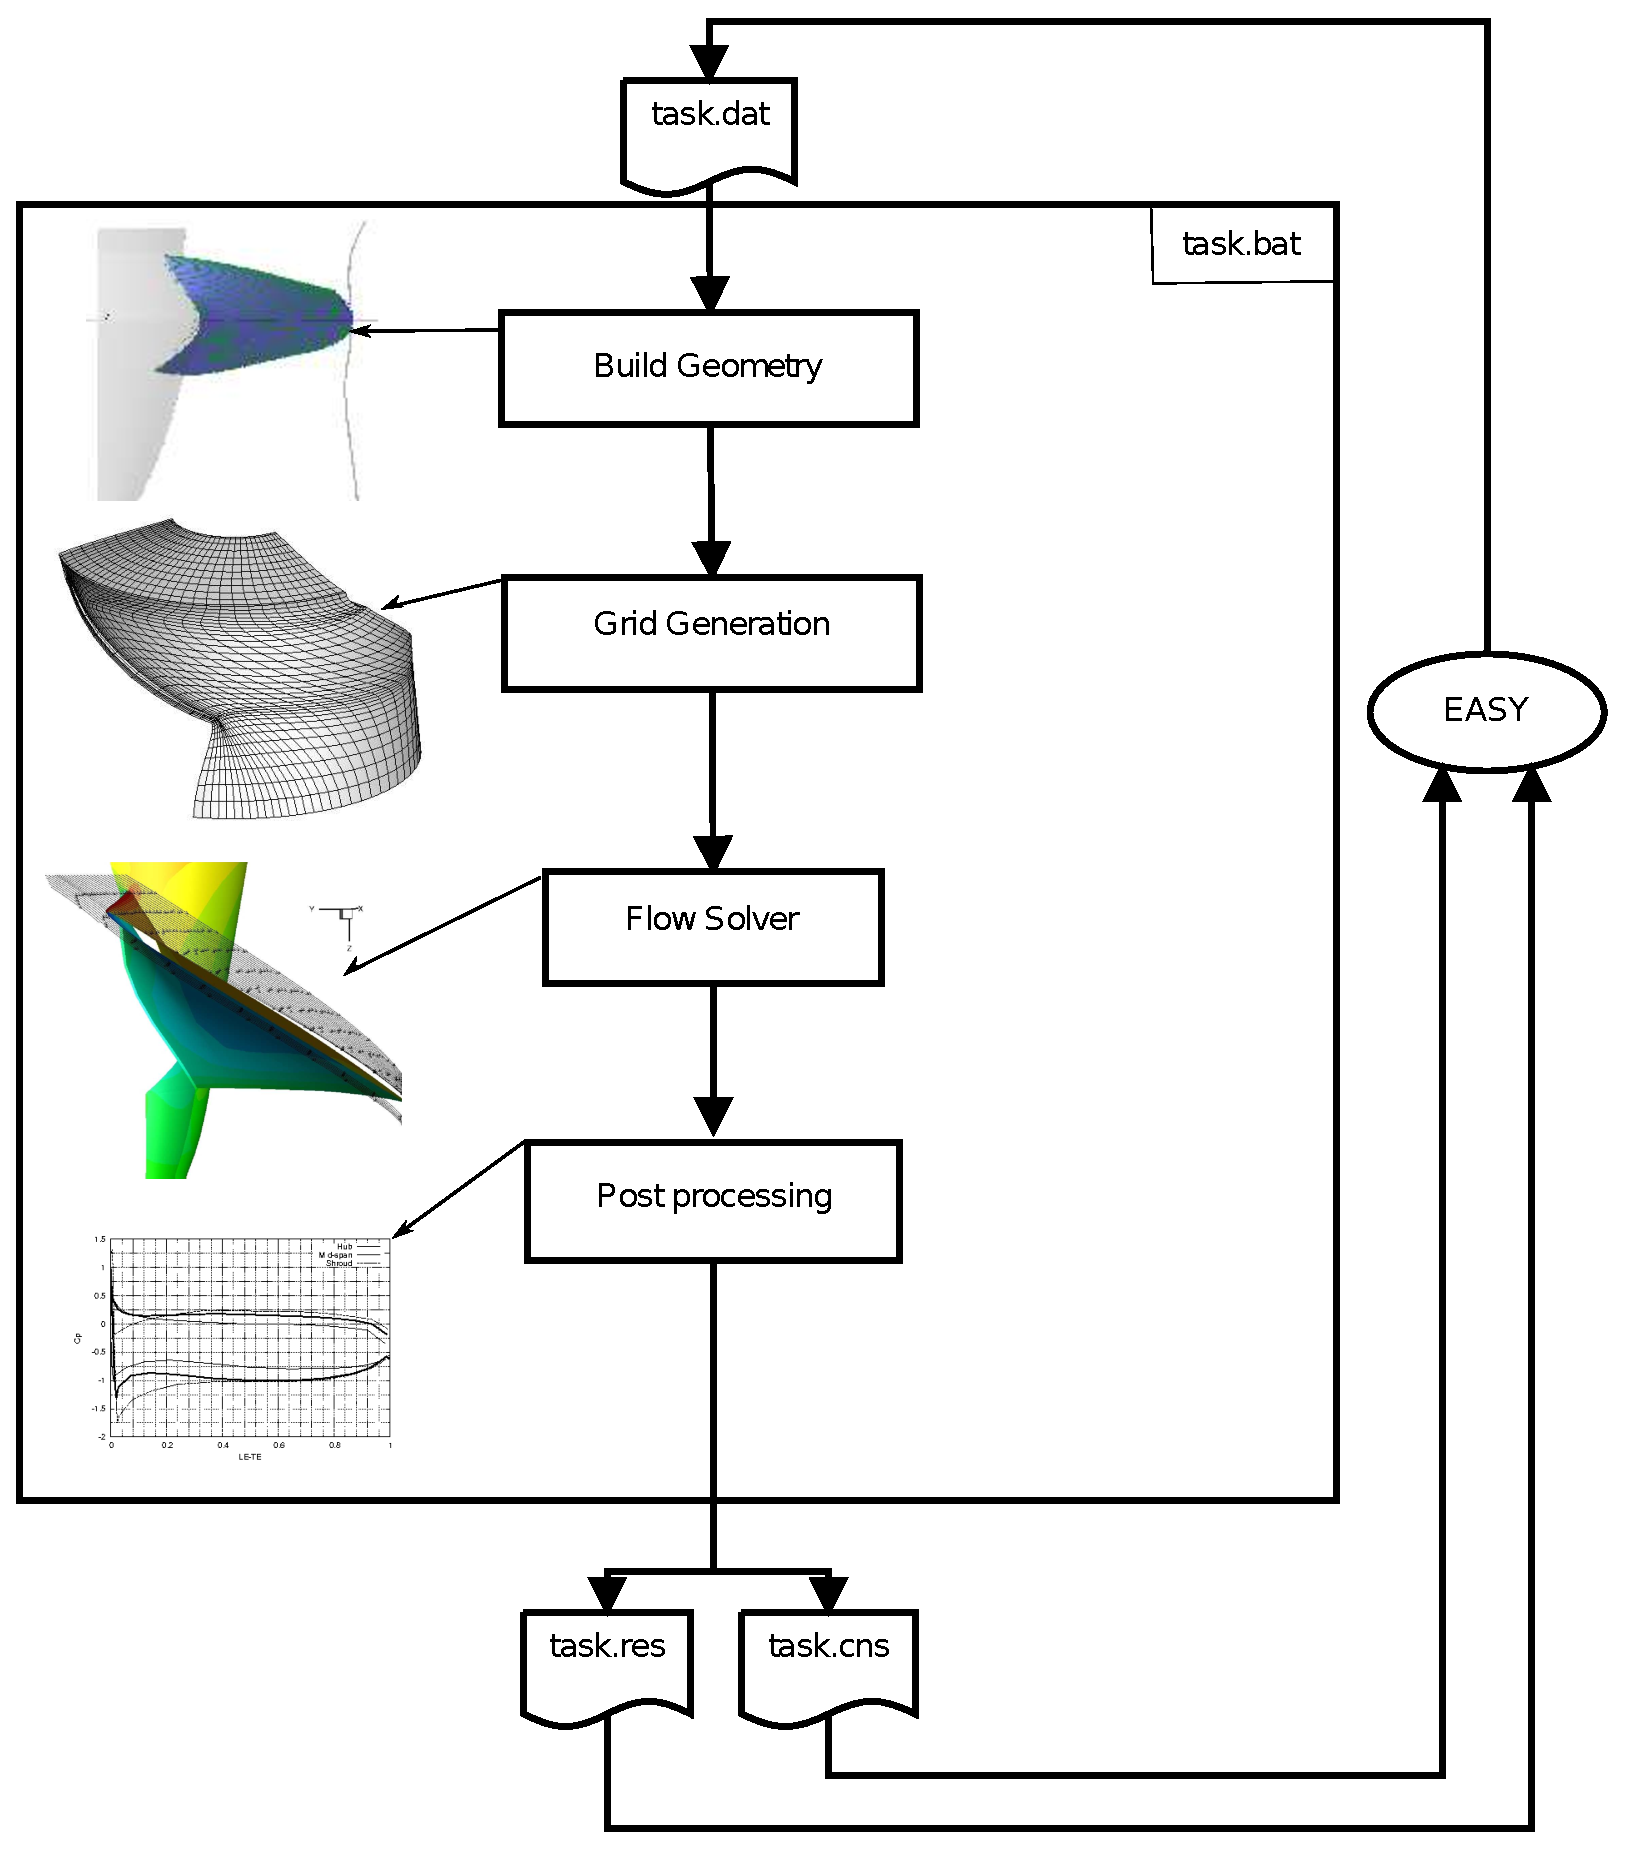
\includegraphics[width=135mm]{Optimizationloop.eps} 
\caption{According to the EASY nomenclature, the evaluation of each new candidate solution provided during the evolution starts by reading the corresponding values of the design variables from the "task.dat" file. A series of codes, being I/O compatible, are sequentially used to finally create the "task.res" and "task.cns" files which indicate the objective and constraint function values respectively. The evaluation process is considered to be terminated once the "task.res" and "task.cns" files  become available to the search engine of EASY. The names of the executable files required for a single evaluation are listed in the script file "task.bat". }
\label{evaltool}
\end{figure}      
      
\section{Evaluation Procedure}
\label{ParamEval}
\subsection{Parameterization for turbine blades}
\label{Paramt}
The  parameterization of a hydraulic turbine blade, of axial, radial or mixed flow type, consists of two steps. The first step is the parameterization of the 3D mean-camber surface. The second step is concerned with the thickness of the blade which is defined by the airfoil shape and the thickness distribution across the blade \cite{dipl_livia,dipl_simon}.

Starting point of the parameterization of the mean-camber surface is its meridional projection. The meridional projection of the mean-camber surface is confined by 4 curves, namely the hub and shroud generatrices, the leading and trailing edge curves (fig.\ref{param1}). All four curves are parameterized by a user-defined number of \Bezier\ points.


%\begin{figure}[h!]
%\centering
%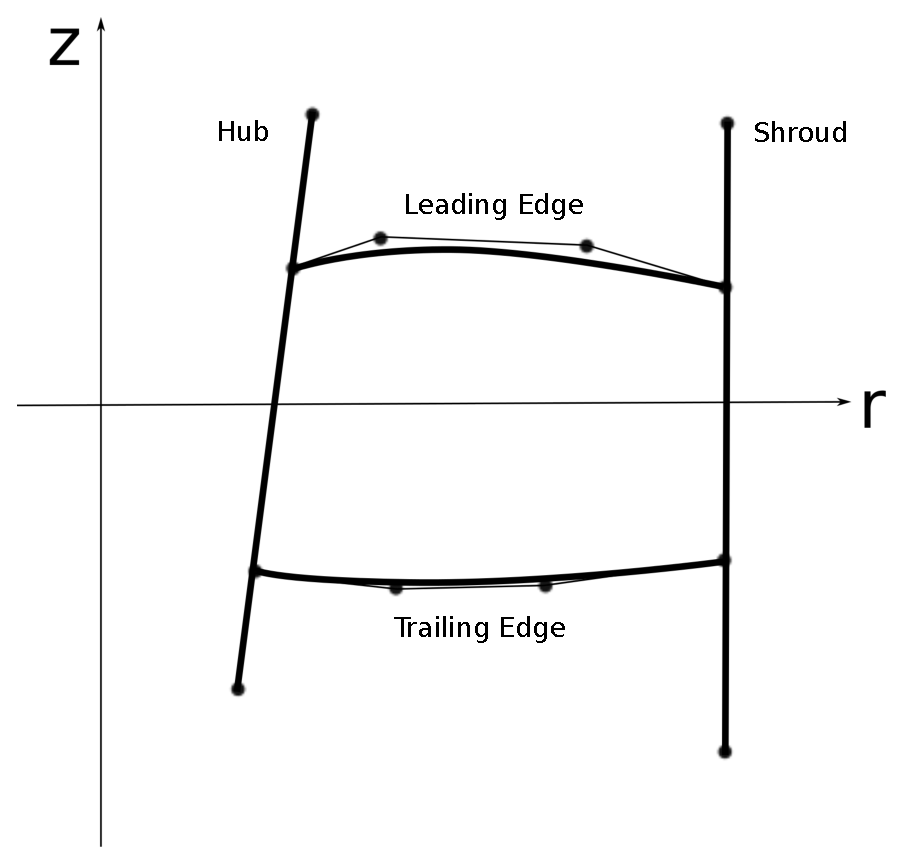
\includegraphics[width=100mm]{param1.eps} 
%\caption{Example of a meridional surface (here a Matrix blade) in cylindrical coordinates (r,z,f=0)}
%\label{param1}
%\end{figure}

Having defined the meridional projection of the mean-camber surface,  the generation of the 3D shape of the mean-camber surface follows. A set of 2D iso-span lines, distributed between the shroud and hub  are generated (fig.\ref{param1}). The 3D shape of the aforementioned lines is  based on their meridional projection and a number of parameters, namely $\rho,\theta,\beta,\zeta$ and $\mu$, which are all defined below. These 3D lines are, then, used as the skeleton of the blade mean-camber surface (fig.\ref{param3}).

\begin{figure}[h!]
\begin{minipage}[b]{0.5\linewidth}
 \centering
 \resizebox*{6.5cm}{!}{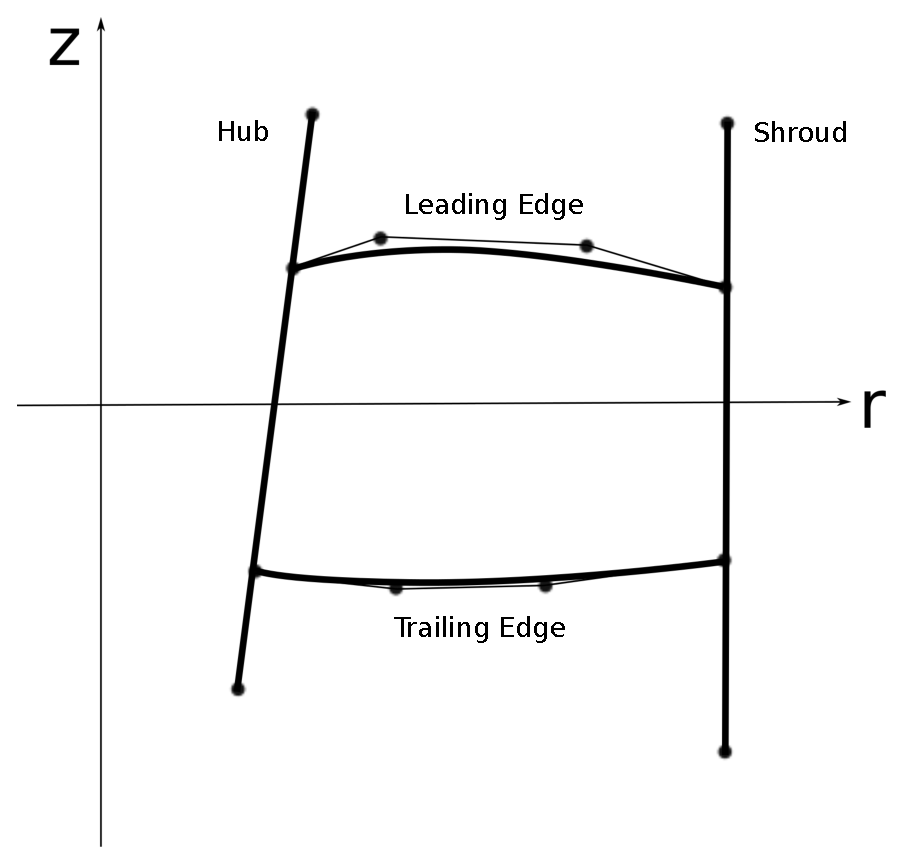
\includegraphics{param1.eps}}
\end{minipage}
\begin{minipage}[b]{0.5\linewidth}
 \centering
 \resizebox*{6.5cm}{!}{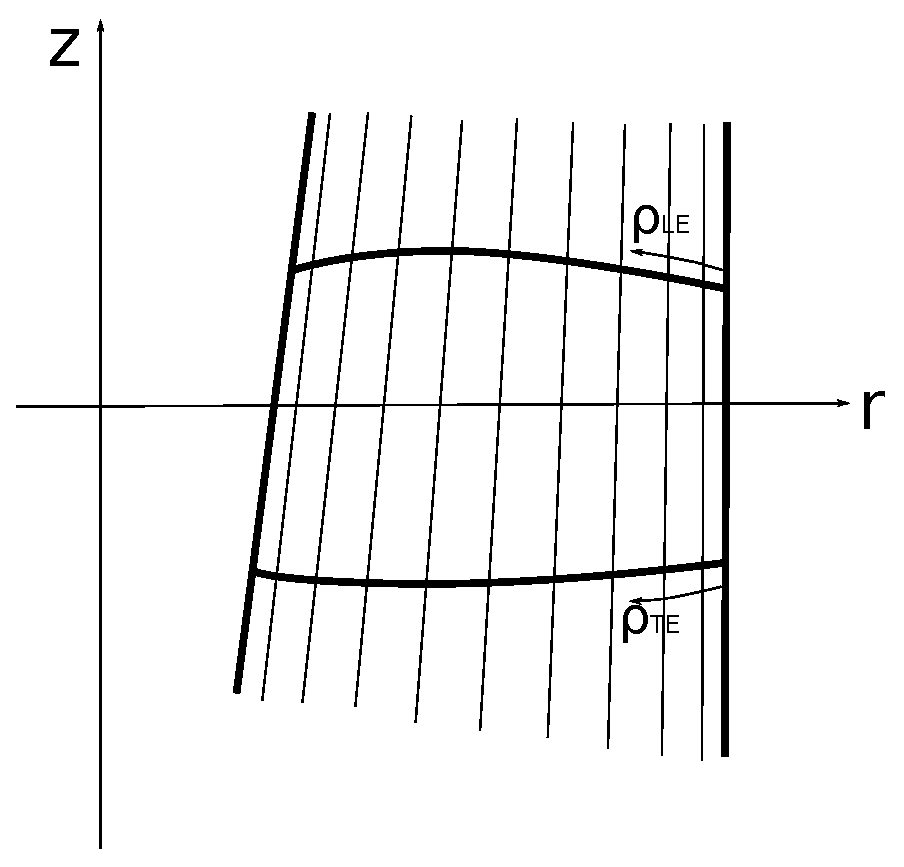
\includegraphics{param2.eps}}
\end{minipage}
\caption{Left: Meridional projection of the mean-camber surface of a HYDROMATRIX$\circledR$ blade. Right: The 2D iso-span lines distributed between shroud and hub. Definition of $\rho$ for the leading and trailing edge.}
\label{param1}
\end{figure}
 

%\begin{figure}[h!]
%\centering
%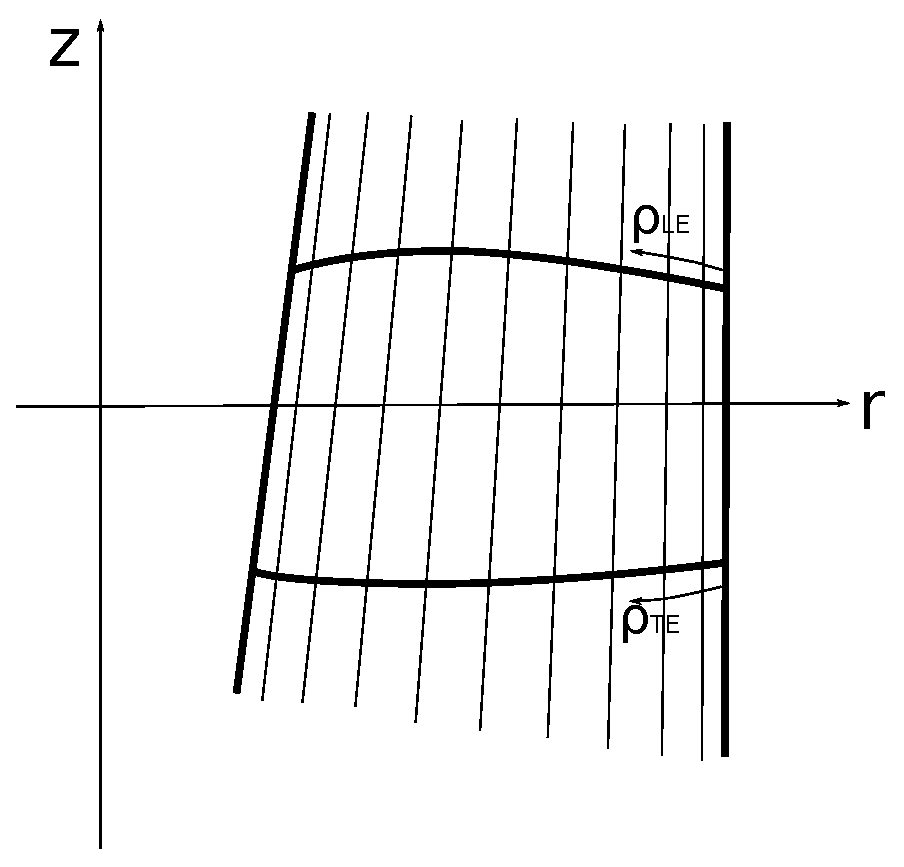
\includegraphics[width=100mm]{param2.eps} 
%\caption{Example of a 2-dimensional streamlines distribution between shroud and hub (here 11 streamlines). %Definition of $\rho$.}
%\label{param2}
%\end{figure}

The $\rho$ value is defined at each point, along both the leading (LE) and trailing (TE) edge, as the normalized meridional projection arc-length of the edge, with zero value at the shroud and unit value at the hub (fig.\ref{param1}). 

\begin{figure}[h!]
\centering
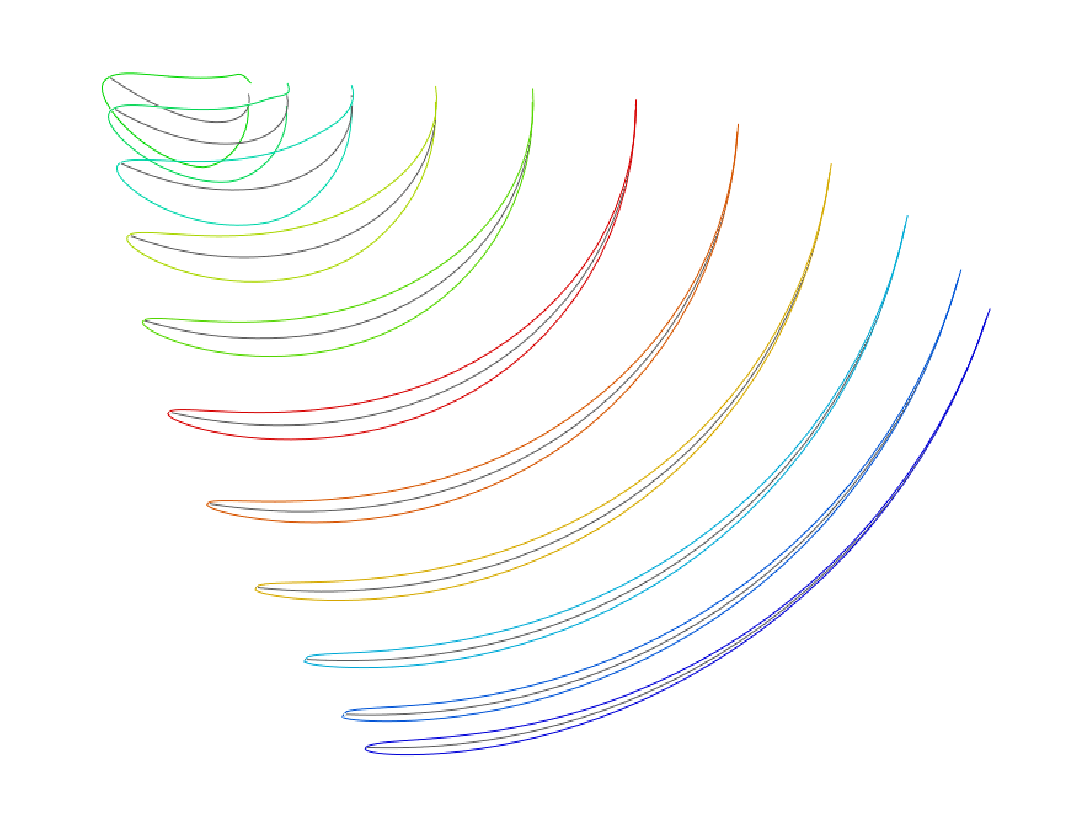
\includegraphics[width=120mm]{param3.eps} 
\caption{The 3D iso-span lines and their superimposed thickness profiles.}
\label{param3}
\end{figure}

The angular position of the LE and TE is controlled by the so-called wrap-around angle $\theta$. % is defined as the angle between the projected linear connection of a mean-surface-point and the z-axis onto the x-y-plane and the x-axis.
$\theta(\rho)$ distributions for the LE and TE together with the r and z values of their meridional projections define the final 3D shape of both edges. On the other hand $\beta$, is defined as the angle between the local tangent to the mean-camber surface and the tangent to the z-centered circle through this point. Therefore, the $\beta(\rho)$ distributions define the mean-camber surface metal angles throughout the previously defined LE and TE. $\beta(\rho)$ and $\theta(\rho)$ distributions are herein parameterized as \Bezier\ curves of a user-defined degree (fig.\ref{param4}).  


\begin{figure}[h!]
\begin{minipage}[b]{1\linewidth}
 \centering
 \resizebox*{14cm}{!}{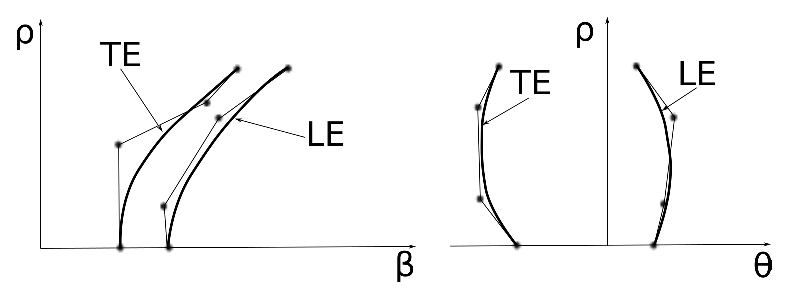
\includegraphics{param4_5.eps}}
\end{minipage}
%\begin{minipage}[b]{0.5\linewidth}
% \centering
% \resizebox*{6.5cm}{!}{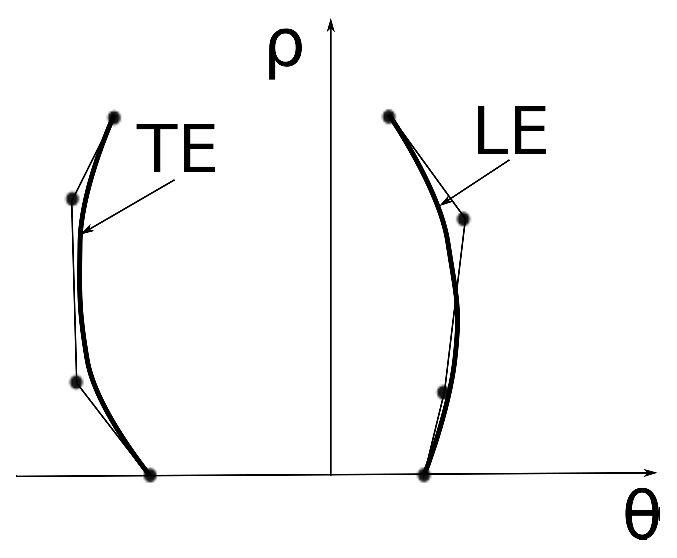
\includegraphics{param5.eps}}
%\end{minipage}
\caption{Left: $\beta(\rho)$ distribution. Right: $\theta(\rho)$ distribution.}
\label{param4}
\end{figure}

The final step in the parameterization of the mean-camber surface is to define its shape between the LE and TE for all the iso-span lines. This is achieved through the conformal mapping $\Phi$


\begin{equation} 
   \Phi:(r,z)\rightarrow \mu, ~~~~\mu=\int{\frac{1}{r}dl}
   \label{phi1} 
\end{equation}
where $l$ denotes the arc-length of the meridional projection of the iso-span line. This conformal mapping performs the transformation of the iso-span lines from cylindrical coordinates $(r,z,\theta)$ to a $(\mu,\theta)$ coordinate system. Herein the iso-span lines (in the $(\mu,\theta)$ coordinate system) are defined by third degree \Bezier\ curves. The first and last control points are fixed on the LE and TE points of each iso-span line and the two internal control points depend on $\zeta_{LE}, ~\zeta_{TE}, ~\beta_{LE}$ and $\beta_{TE}$ angles, respectively (fig.\ref{param7}).
  
Finally, the $\zeta(\rho)$ distributions, one for the LE ($\zeta_{LE}$) and another for the TE ($\zeta_{TE}$) define the position of the two internal control points for all the iso-span lines ($0\leq\rho\leq1$). Therefore, the $\zeta$ distributions can be seen as the curvature control system of the aforementioned parameterization of the mean-camber surface scheme, since it defines how strongly the $\beta$ values at LE and TE affect the $\beta$ values in the interior of the mean-camber surface. Similar to $\theta(\rho)$ and $\beta(\rho)$ also $\zeta(\rho)$ distributions are parameterized as \Bezier\ curves of a user-defined degree (fig.\ref{param7}). The inverse conformal mapping $\Phi^{-1}$ is, then, used to transform the iso-span lines from the $(\mu,\theta)$ coordinate system back to the cylindrical one. 

\begin{figure}[h!]
\begin{minipage}[b]{1\linewidth}
 \centering
 \resizebox*{14cm}{!}{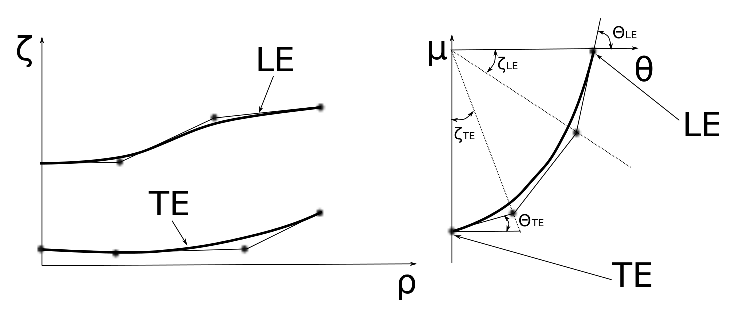
\includegraphics{param6_7.eps}}
\end{minipage}
%\begin{minipage}[b]{0.5\linewidth}
% \centering
% \resizebox*{7.5cm}{!}{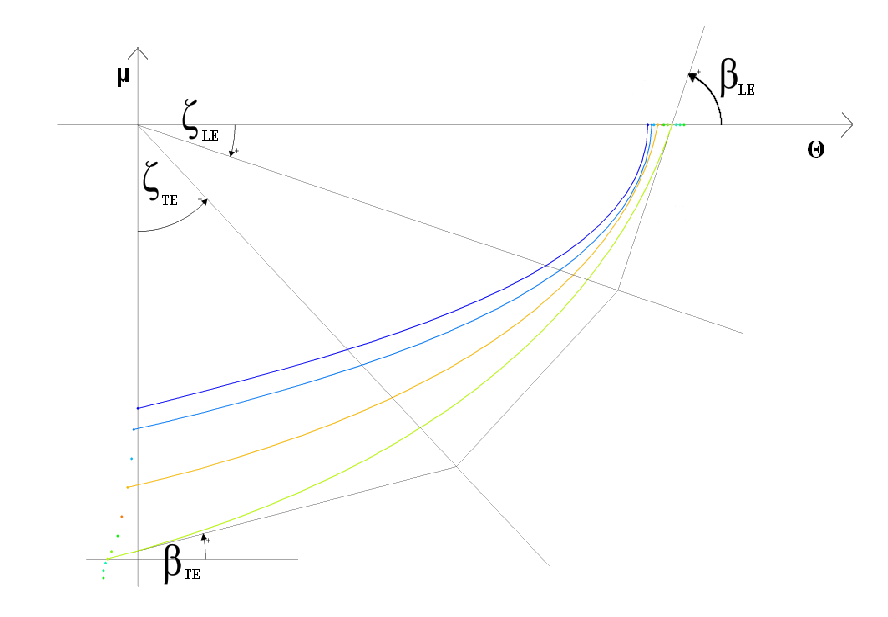
\includegraphics{param7.eps}}
%\end{minipage}
\caption{Left: $\zeta(\rho)$ distributions for $\zeta_{LE}$ and $\zeta_{TE}$. Right: Iso-span line, in the $(\mu,\theta)$ coordinate system, and its \Bezier\ control point polygon.}
\label{param7}
\end{figure}

The airfoil profiles are defined by a user-defined number of \Bezier\ points (fig.\ref{param8}) and the absolute thickness by two thickness (t($\rho$)) distributions (fig.\ref{param10}) (separately for the SS and PS). Airfoil profiles are scaled for their maximum thickness to be equal to the one specified by the t($\rho$) distribution. The scaled airfoil profiles are, then, superimposed onto the mean-camber surface to create the final 3D blade (fig.\ref{param10}).  

\begin{figure}[h!]
\centering
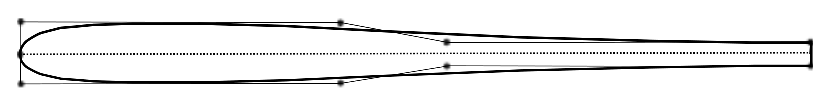
\includegraphics[width=150mm]{param8.eps} 
\caption{\Bezier\ control point polygons for the PS and SS.}
\label{param8}
\end{figure}

%\begin{figure}[h!]
%\centering
%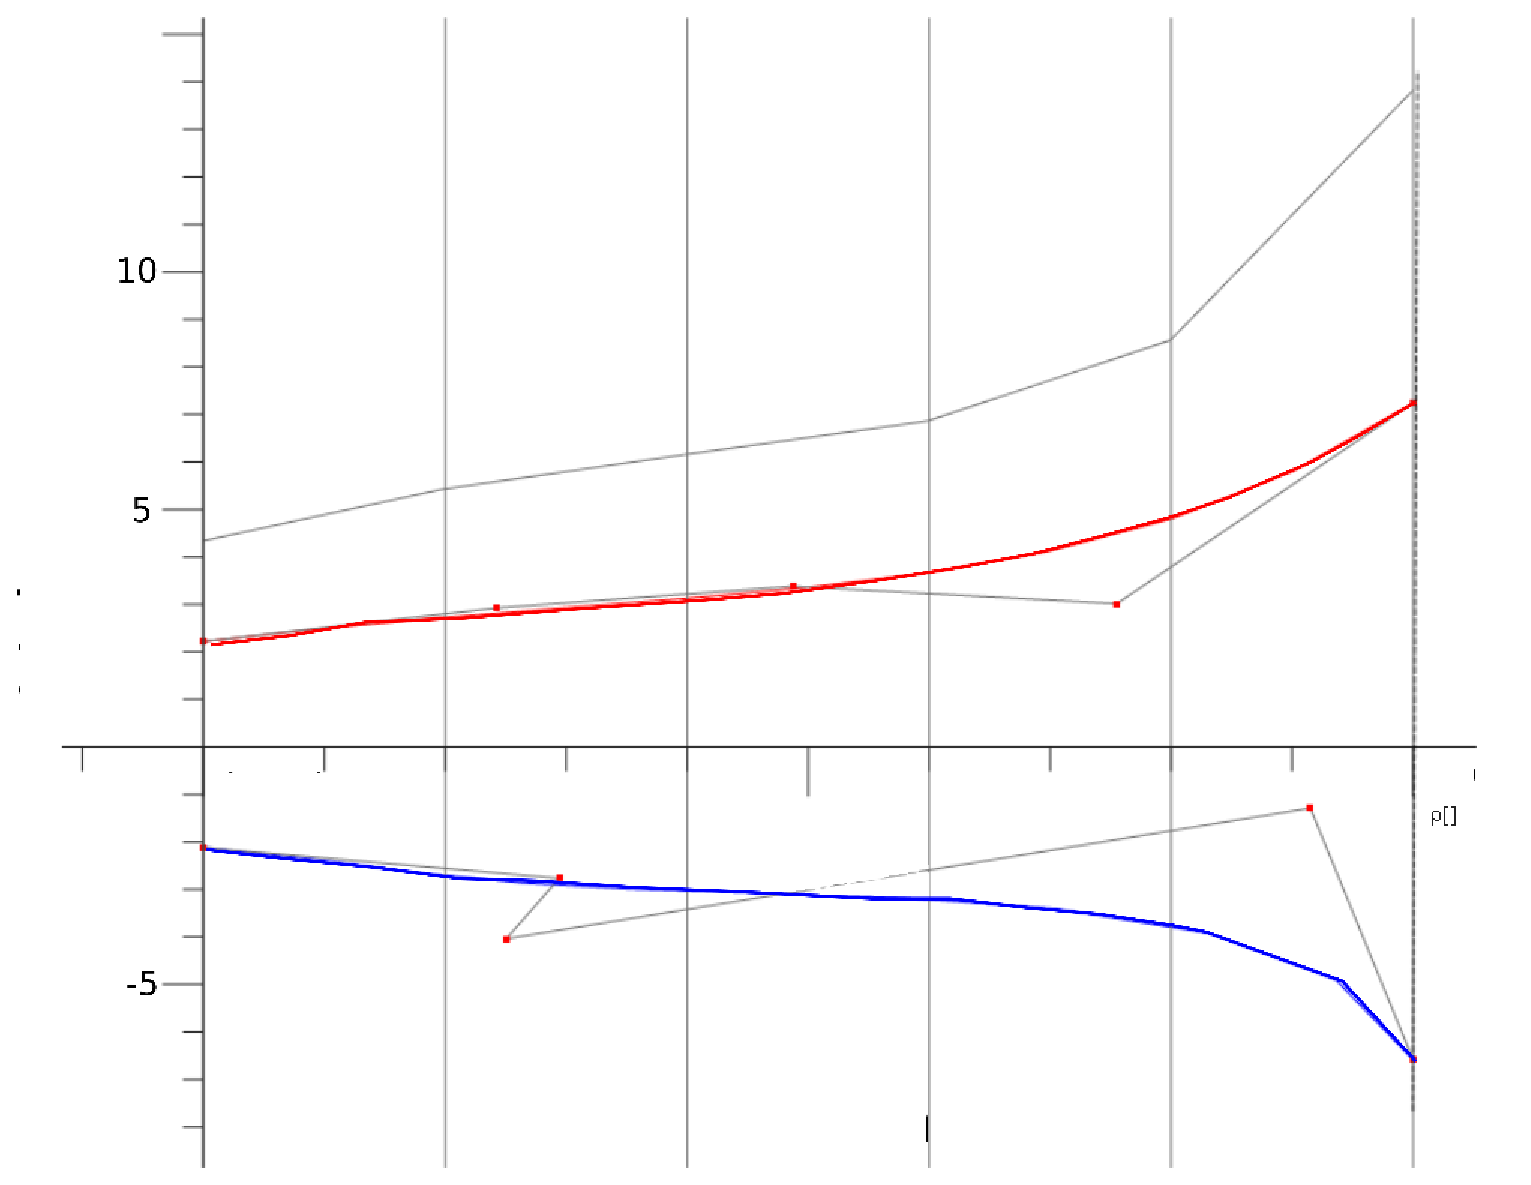
\includegraphics[width=60mm]{figure5.eps} 
%\caption{thickens-$\rho$ distribution.}
%\label{param9}
%\end{figure}


\begin{figure}[h!]
\begin{minipage}[b]{0.5\linewidth}
 \centering
 \resizebox*{6.5cm}{!}{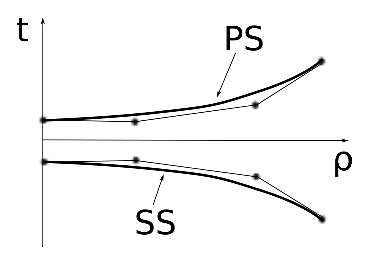
\includegraphics{param9.eps}}
\end{minipage}
\begin{minipage}[b]{0.5\linewidth}
 \centering
 \resizebox*{6.5cm}{!}{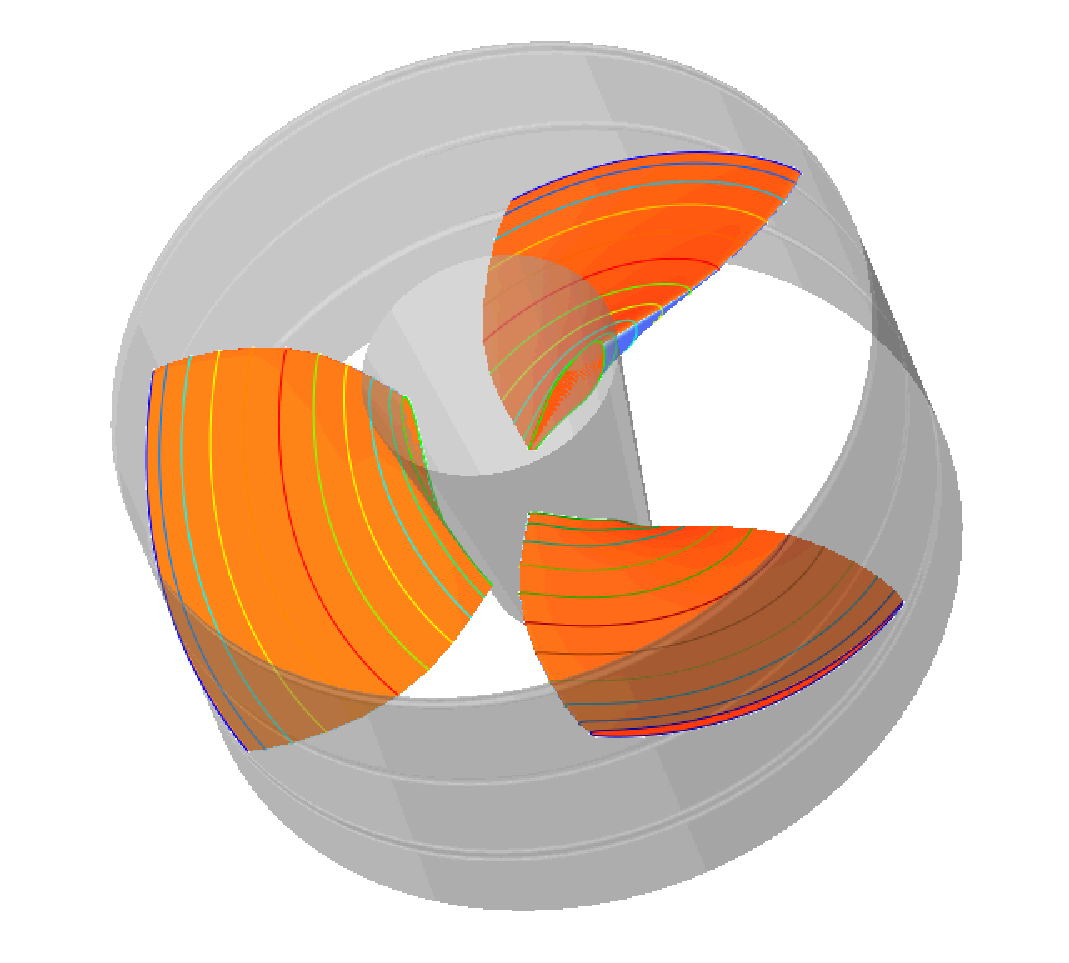
\includegraphics{param10.eps}}
\end{minipage}
\caption{Left: t($\rho$) distribution. Right: 3D geometry of a HYDROMATRIX$\circledR$ turbine with three blades.}
\label{param10}
\end{figure}

\subsection{Space discretization - Grid generation}
\label{SpaceDisct}
A tailor-made for hydraulic turbomachines multi-bloc structured grid generator is used. This is able to handle axial, radial and mixed flow machines. Structured grids, using blocks with fixed topology can, via stretching and twisting them, create grids that fit the geometries under consideration. A multi-block topology (several interconnected structure grid blocks) gives maximum freedom to the user for generating grids around quite complex geometries (fig.\ref{grid1}). 


\begin{figure}[h!]
\centering
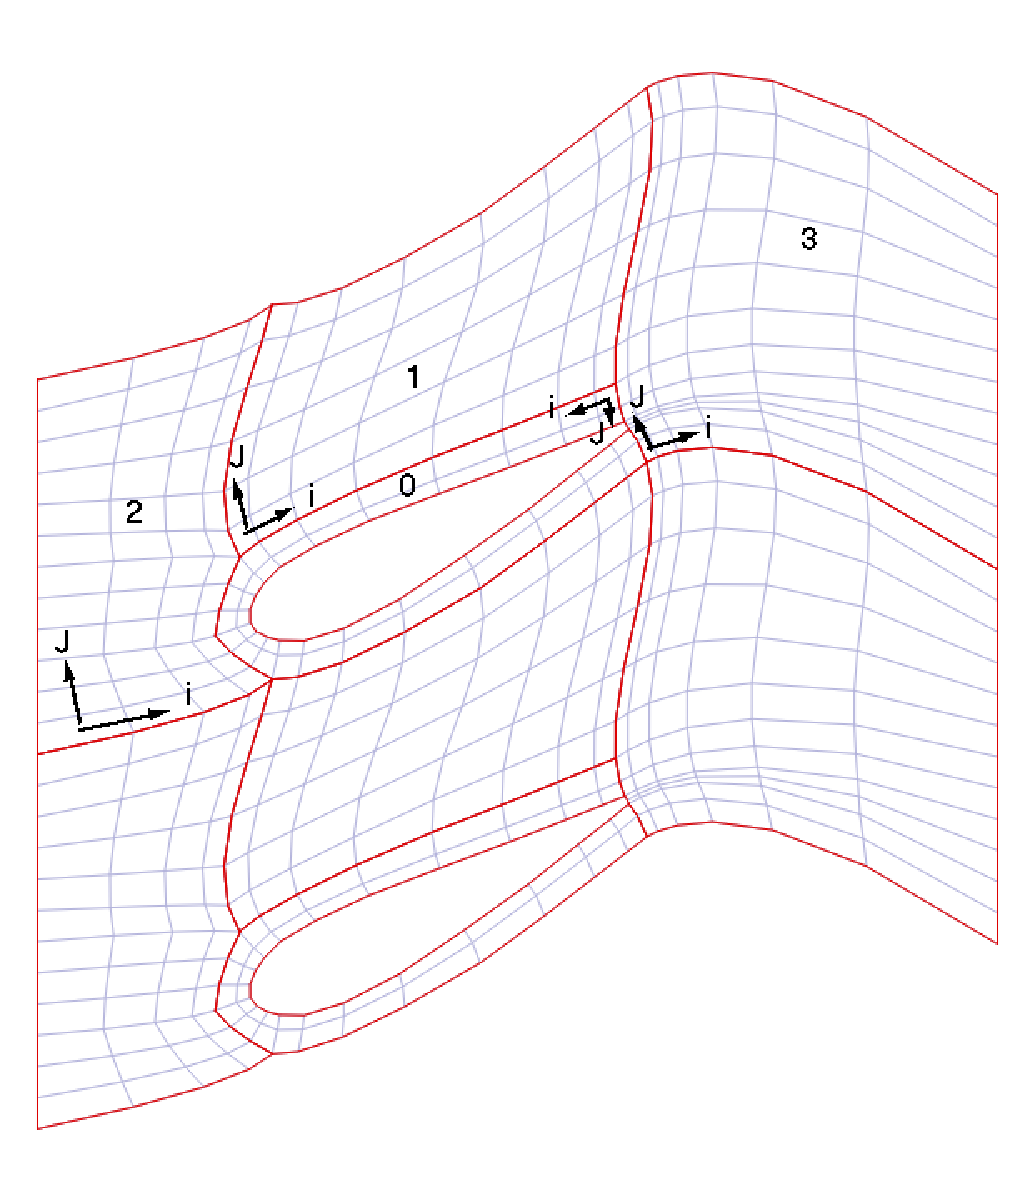
\includegraphics[width=100mm]{cGridSkBlockIndex.eps} 
\caption{The four-block topology of a hydraulic turbine. In the sake of simplicity, this is shown on the blade-to-blade grid at mid-span. Block 0 is of C-type and is used to discretize the area in the vicinity of the blade (herein airfoil). Blocks 1 to 3 are of rectangular type and are used to fill the space from pressure side to suction side, between blade LE and inlet and  blade TE and outlet respectively. }
\label{grid1}
\end{figure}


In this thesis, with respect to the topological characteristics of hydraulic turbo-machines, such as the the TE thickness and the extensions towards the inlet and outlet of the domain, a four-block topology is used  fig. \ref{grid1}. Block 0 is of C-type and is used to mesh the area in the vicinity of the blade, capturing the TE thickness. Block 1 fills the space between two consecutive blades. Block 2 fills the space from the inlet to the blade LE. Finally, Block 3 fills the space after blocks 0 and 1 up to the outlet. 

Here the user may control the grid via changing the shape of the block edges, defining number of nodes at each location (fig.\ref{grid2}) and  the distribution of grid-nodes at the domain-borders (fig.\ref{grid3}).                      


\begin{figure}[h!]
\centering
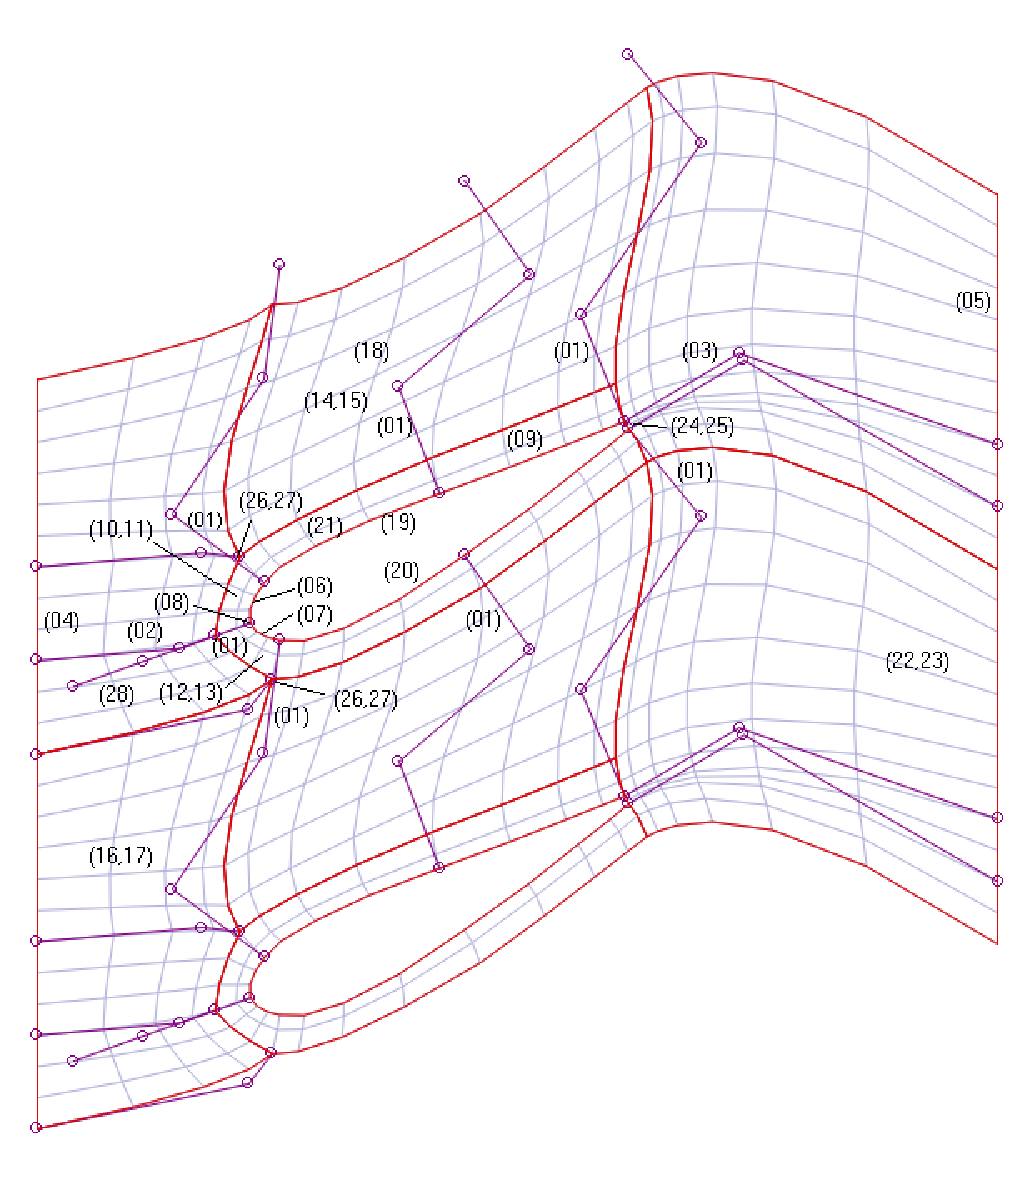
\includegraphics[width=100mm]{cGridSkParam.eps} 
\caption{User-defined parameters controlling the shape of the block edges. These are a set of values constructed from a number of angles and distances that defined the control points of the figure. Numbers on these figure correspond to the number of the parameters and are depicted in the domains that they influence.}
\label{grid2}
\end{figure}

\begin{figure}[h!]
\centering
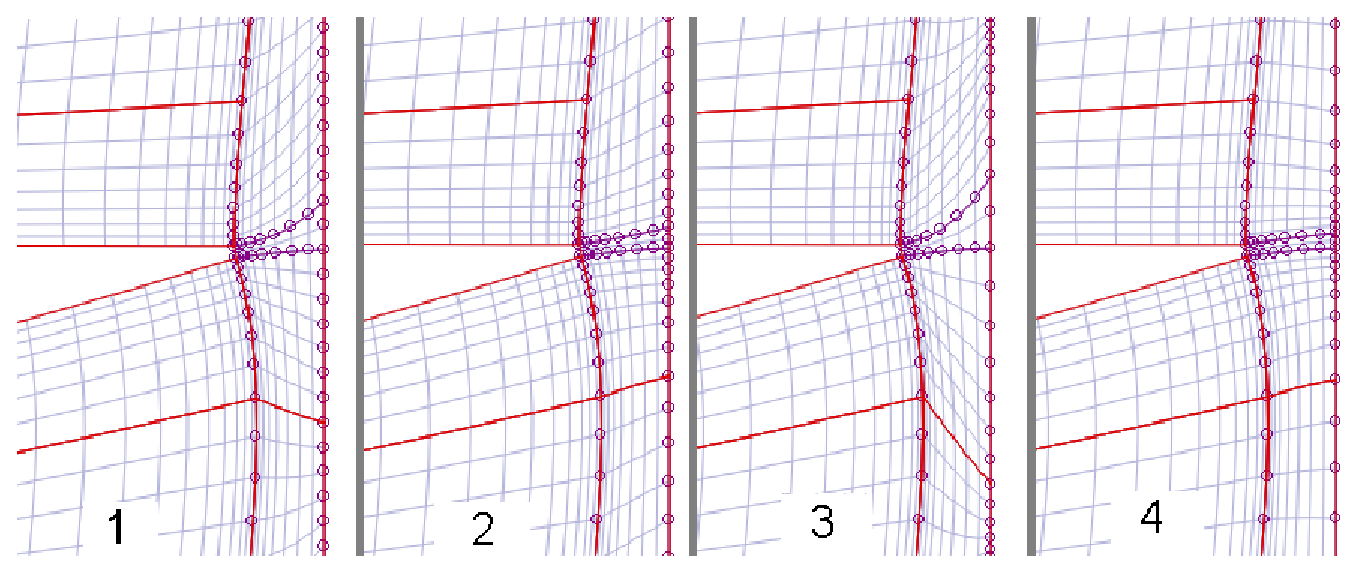
\includegraphics[width=120mm]{sketchDistrEast.eps} 
\caption{Parameters controlling the distribution of grid-nodes along the domain-boundaries allow the user to place a greater number of points in regions of high gradients while reducing the number of grid nodes in regions with small gradients.}
\label{grid3}
\end{figure}

To construct the three-dimensional grid a user-defined number of pseudo two-dimensional (laying on iso-span surfaces fig \ref{grid4}) grids are computed using the grid parameterization as described above and are then combined to create the final 3D grid.

\begin{figure}[h!]
\centering
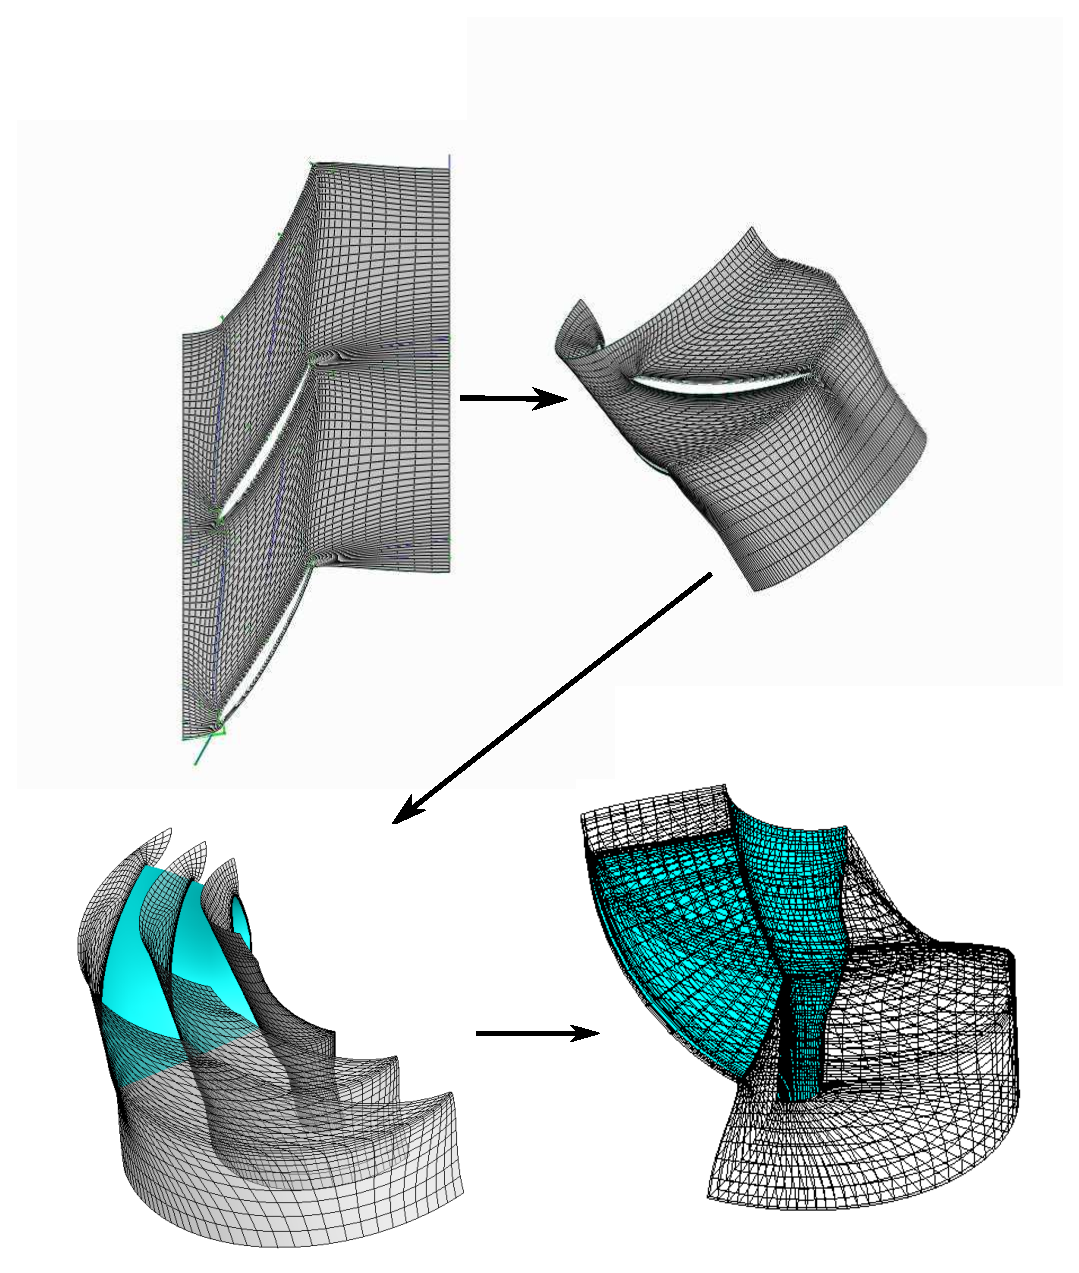
\includegraphics[width=140mm]{merid.eps} 
\caption{Iso-span surface grid as pseudo-2D grid. A user-defined number of the iso-span surface grids (from hub to shroud) is combined in order to generate the three-dimensional grid. Top Left: the pseudo-2D grid at the mid-span position. Top Right: the same grid transformed buck to the 3D space. Bottom Left: The hub: mid-span and shroud grids. Bottom Right: Final grid.}
\label{grid4}
\end{figure}

It is important to mention that the described grid generation technique can accommodate a great variation of geometries without failing. This is of great importance for a grid technique to be used in an optimization framework. Good geometries should under no circumstances be classified as "failed" due to the failure of the grid generation process. 

In this thesis both, guide vane and runner blade channels are meshed using a grid generation tool, with the previous features, developed by Andritz-ASROE. 
%Typically, for speed sake, only one circumferential channel is computed (one guide vane and one runner channel with mixing plane interface).  

\FloatBarrier
\subsection{Flow Solver}
\label{FlowSolvert}
Water flow through the hydraulic turbine blades is simulated by a CFD code developed by Andritz-ASROE. The aforementioned code is a multiblock solver for incompressible 3D euler flow. The Euler (eq. \ref{Euler1}) equations are expanded by an artificial compressibility, the solution is achieved, using the 1D Roe approximate Riemann solver \cite{Roe81}, iteratively by ADI (alternating direction implicit) method on structured grids. Convergence is accelerated by a V-cycle multigrid schema. The solver is developed for hydraulic turbomachines, rotational axis is z-axis.

%using the 1D Roe approximate Riemann solver \cite{Roe81}
%is solving the Euler equations (eq. \ref{Euler1}) based on the artificial compressibility approach using the 1D Roe approximate Riemann solver \cite{Roe81}. For sake of wall time reduction this code employs a multi-grid solver. 

In differential form the Euler equations (artificial compressibility approach) are;
\begin{equation} 
    \frac{\partial Q}{\partial t}=\nabla \cdot F
	\label{Euler1}
\end{equation}

where,
\begin{eqnarray}
		Q= \left( {\begin{array}{c}
 		p    \\
 		u_1  \\
 		u_2  \\
 		u_3  \\
 		\end{array} } \right)
 		F_i= \left( {\begin{array}{c}
 		\beta ^2 u_i    \\
 		\beta ^2 u_1u_i + p\delta _1^i  \\
		\beta ^2 u_2u_i + p\delta _2^i  \\
 		\beta ^2 u_3u_i + p\delta _3^i  \\
 		\end{array} } \right)
\label{Euler3}
\end{eqnarray} 
 
where $\beta$ the artificial compressibility \cite{Chorin,Turkel87} and $\delta^i_j$ the Kronecker symbol.

The boundary conditions regarding inlet and outlet, for the herein used solver, are applied in an explicit way on grouped faces via the phantom cell technique. This are;
\begin{itemize}
\item[\textbf{Inlet: }]
	\begin{itemize}
	\item total pressure profile and velocity angle;
	\item or velocity profile;
	\end{itemize}
\item[\textbf{Outlet: }]
	\begin{itemize}
	\item static pressure;
	\item or static pressure and radial equilibrium;
	\item or total pressure and radial equilibrium;
	\end{itemize}
\end{itemize}

Any combination using the ``velocity profile'' inlet boundary results in a given massflow and the Hydraulic head  is a result form the solution of the flow equations. On the the other hand, if the ``total pressure profile and velocity angle'' inlet boundary condition is used in combination with the ``total pressure and radial equilibrium'' outlet  boundary condition then the Hydraulic head is given and the massflow is resulting from the solution of the flow equations. The choice of either configuration plays a significant role in the operating point control as will be shown later on.        
%Using the above formulation each CFD calculation inside one runner channel takes only a few minutes. This fact and the observation that the influence of turbulence and viscosity are small enough allows, in combination with the proposed in this thesis techniques, the use of EAs as design tools in an industrial level i.e. with short (acceptable in a industrial environment) wall time. 

%Of coarse for the above statement to be true the appropriate objective functions, derived out of quality metrics that reflect the real quality of a runner and are not significantly influenced by turbulence and viscosity, have to be chosen. This type of metrics are presented, in detail, in section \ref{metrics} and will be used throughout this chapter. 
 
%In order to eliminate the obvious problem for incompressible flow (reduced state equation) an %artificial compressibility is introduced (cite R2 S5 ,maybe more). 

%The term $\frac{\partial \rho}{\partial t}$ is expanded by $\frac{\partial p}{\partial p}$, which results in 


%\begin{eqnarray}
%	\frac{\partial \rho}{\partial t} = \frac{\partial \rho}{\partial t}\frac{\partial p}{\partial p}
% = \frac{\partial p}{\partial t}\frac{1}{(\frac{\partial p}{\partial \rho})} 
% = \frac{\partial p}{\partial t}\frac{1}{\beta ^2}    
%\end{eqnarray}

%Thus the artificial compressibility $\beta$ is defined as;

%\begin{eqnarray}
%	\beta=\sqrt{\frac{\partial p}{\partial \rho}}
%\end{eqnarray}



\section{Hydraulic turbine-runner quality metrics}
\label{metrics}
The metrics used so as to quantify the quality of the candidate solutions are presented below. A metric may coincide with a objective function or part of an objective function or a constraint used in the optimization problem.

In this thesis metrics are associated with:
\begin{itemize}
\item{\textbf{$\sigma$:}} The cavitation behaviour of the blade in hand; cavitation is a common problem of all hydraulic machine subject to low pressure liquids, causing performance degradation and structural damages.
\item{\textbf{M1}} The Circumferential and meridional velocity profiles at the exit position of the runner; the exit of the runner coincides with the inlet to the draft-tube and these profiles significantly affect the matching of the two components.
\item{\textbf{M2}} The blade loading quality, since equidistributed loading is desired along the chordwise direction of the blade at any span-wise location.
\item{\textbf{M3}} The pumping surface of the blade; in case of non-regulated turbines neither the stator nor the rotor blade can be rotated/adjusted to operate optimally at every operating point. In such a case, during  part load operation, a small part of the blades surface is operating as a pump, i.e. pressure side has lower pressure than suction side, this surface is desired to be minimized.
\end{itemize}


\subsection{Cavitation metric}
\label{cav.metric}
Cavitation in hydraulic turbines, is the phenomenon of water vaporization (formation of cavities/bubbles) as the pressure tends to become lower than the vapour pressure. When the cavitation bubbles collapse in the vicinity of a solid surface, they can cause erosion, compromising thus both the structural integrity (removed material) and the hydraulic performance (altered shape) of the machine \cite{thiruvengadam1974handbook,knapp1970cavitation,brennen1995cavitation}.  In addition, the collapse of cavitation bubbles generates noise, via the large, momentary, pressures that are generated when the internal of the bubble is highly compressed.

The conventional way to characterize how close the minimum liquid pressure is to the vapour pressure and, therefore, quantify the danger of cavitation to occur, is by means of the so-called cavitation number $\sigma$, defined as,

\begin{eqnarray}
		\sigma=\frac{p_{\infty}-p_{v,T_{\infty}}}{0.5\rho_{L}U^2_{\infty}}
\label{Cavi}
\end{eqnarray}
where, $U_{\infty}$,$p_{\infty}$ and $T_{\infty}$ are a reference velocity, pressure and temperature respectively. $\rho_{L}$ is the liquid density and $p_{v,T_{\infty}}$  is the saturated vapour pressure. 

Clearly if $\sigma$ is sufficiently large, $p_{\infty}$ is large compared with $p_{v,T_{\infty}}$ or $U_{\infty}$, single-phase liquid flow will occur. However, if $\sigma$ drops below the $\sigma$ incipient ($\sigma_i$) value cavitation will occur. In the simplified case of a liquid that cannot withstand any tension and in which vapour bubbles appear instantaneously when minimum pressure ($p_{min}$) reaches $p_{v}$,

\begin{eqnarray}
		\sigma_i=\frac{p_{\infty}-p_{min}}{0.5\rho_{L}U^2_{\infty}}
\label{Cavi2}
\end{eqnarray}
Hence, the incipient cavitation number could be ascertained from observations, measurements or simulations of the single-phase flow i.e. for $\sigma > \sigma_i$ the pressure along the entire flow filed is greater than $p_v$ thus no cavitation occurs. On the other hand, if $\sigma \leq \sigma_i$, it exists at least one point in the flow filed with pressure lower than $p_v$ thus cavitation does occur. 


In the case of hydraulic turbines the tendency of the flow to cavitate is characterized by the so called Thoma cavitation coefficient $\sigma$, 
\begin{eqnarray}
		\sigma=\frac{p_{tot,exit}-p_{v}}{\rho_{L}gH}
\label{Cavi3}
\end{eqnarray}
where $p_{tot,exit}$ is the total pressure at the exit of the turbine, $p_v$ the vapour pressure for the liquid and $H$ the hydraulic turbine head. The denominator is the total pressure difference between the turbines inlet and outlet.   

Making the same assumptions as for eq.\ref{Cavi2} the $\sigma_i$ for the Thomas cavitation coefficient  is, 

\begin{eqnarray}
		\sigma_i=\frac{p_{tot,exit}-p_{min}}{\rho_{L}gH}
\label{Cavi4}
\end{eqnarray}

Let $C_p$ the pressure coefficient for hydraulic turbines be 
\begin{eqnarray}
		C_p=\frac{p-p_{tot,exit}}{\rho_{L}gH}
\label{Cpdef}
\end{eqnarray}

The $\sigma_i$ for the Thomas cavitation coefficient can be described as 
\begin{eqnarray}
		\sigma_i=-C_{pmin}
\label{Cavi6}
\end{eqnarray}
where $C_{pmin}$ is the $C_p$ value at the location with minimum pressure ($p_{min}$).

The cavitation behaviour of a hydraulic turbine can be observed through the $C_p$ distribution as they are plotted over the hydraulic turbine surfaces.  In fig. \ref{design-cav-cp} the $C_p$ distribution regarding the turbine runner blade at mid-span position is depicted. The three indicative scenarios for this case is; a) $\sigma>-C_{pmin}$ thus $p_v<p_{min}$ and therefore cavitation dose not occur; b)  $\sigma=-C_{pmin}$, in which case if the assumptions of eq.\ref{Cavi2} and \ref{Cavi4} are true, the liquid cannot withstand any tension and vapour bubbles appear instantaneously when minimum pressure ($p_{min}$) reaches $p_{v}$, cavitation will occur at the point of minimum pressure; and c) $\sigma<-C_{pmin}$ in which case $p<p_v$ over a portion of the chord, in the case of the chordwise distribution depicted in fig. \ref{design-cav-cp}, or area, in the case of the complete blade. This region is, therefore, considered cavitated.     

\begin{figure}[h!]
\begin{minipage}[b]{1\linewidth}
 \centering
 \resizebox*{14cm}{!}{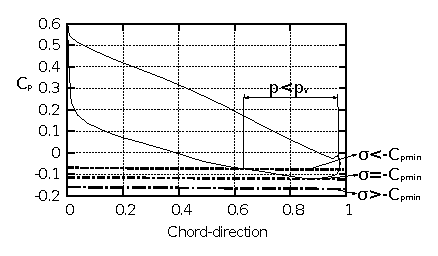
\includegraphics{CP2.eps}}
\end{minipage}
\caption{Pressure coefficient distribution for the mid-span position.}
\label{design-cav-cp}
\end{figure}

In this thesis, in order to reduce the effects of the assumptions of eq.\ref{Cavi2} and eq.\ref{Cavi4}, the $\sigma$-Histogram method \cite{Schmidl} is used. In $\sigma$-Histogram method, during the calculation of $\sigma_i$ the minimum pressure $p_{min}$ is replaced with so called histogram pressure ($p_{Hist}$) (eq. \ref{Cavi7}). $p_{Hist}$ is extracted from the blade pressure distribution where a user-defined surface percentage (A) is required to have pressure values below $p_{Hist}$ fig.\ref{design-cav-histo}.  

\begin{eqnarray}
		\sigma_i^{Hist}=\frac{p_{tot,exit}-p_{Hist}}{\rho_{L}gH}
\label{Cavi7}
\end{eqnarray}
%where

%\begin{eqnarray}
%		A(p<p_{Hist})=A\%A_{Blade}
%\label{Cavi7}
%\end{eqnarray}

\begin{figure}[h!]
\begin{minipage}[b]{1\linewidth}
 \centering
 \resizebox*{14cm}{!}{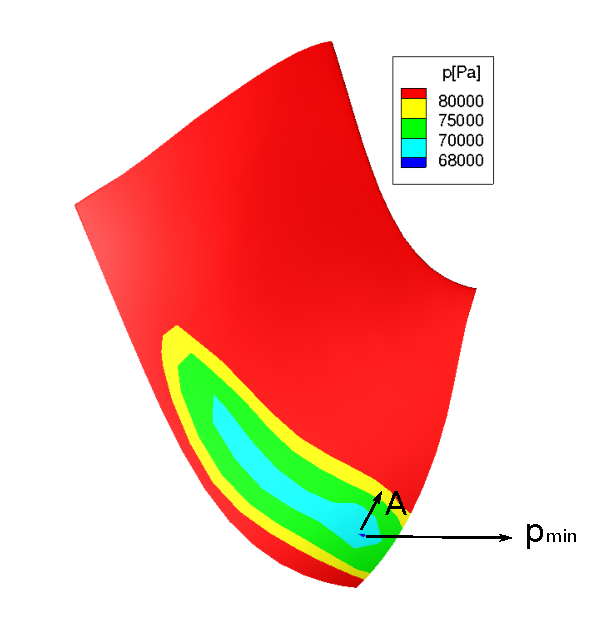
\includegraphics{histo.eps}}
\end{minipage}
\caption{$p_{Hist}$ computed with three different A values is depicted here along side with $p_{min}$ on the suction side of a Francis hydraulic turbine. Increasing A results in increased $p_{Hist}$ and therefore reduced $\sigma_i^{Hist}$. A values in this figure are exaggerated for sake of presentation.}
\label{design-cav-histo}
\end{figure}

%\begin{figure}[h!]
%\begin{minipage}[b]{0.5\linewidth}
% \centering
% \resizebox*{7.5cm}{!}{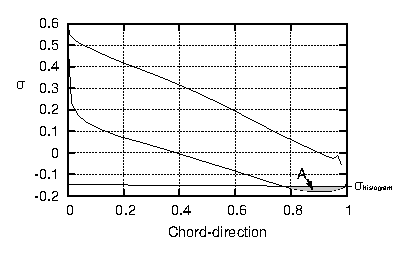
\includegraphics{sigma.eps}}
%\end{minipage}
%\begin{minipage}[b]{0.5\linewidth}
% \centering
% \resizebox*{6.0cm}{!}{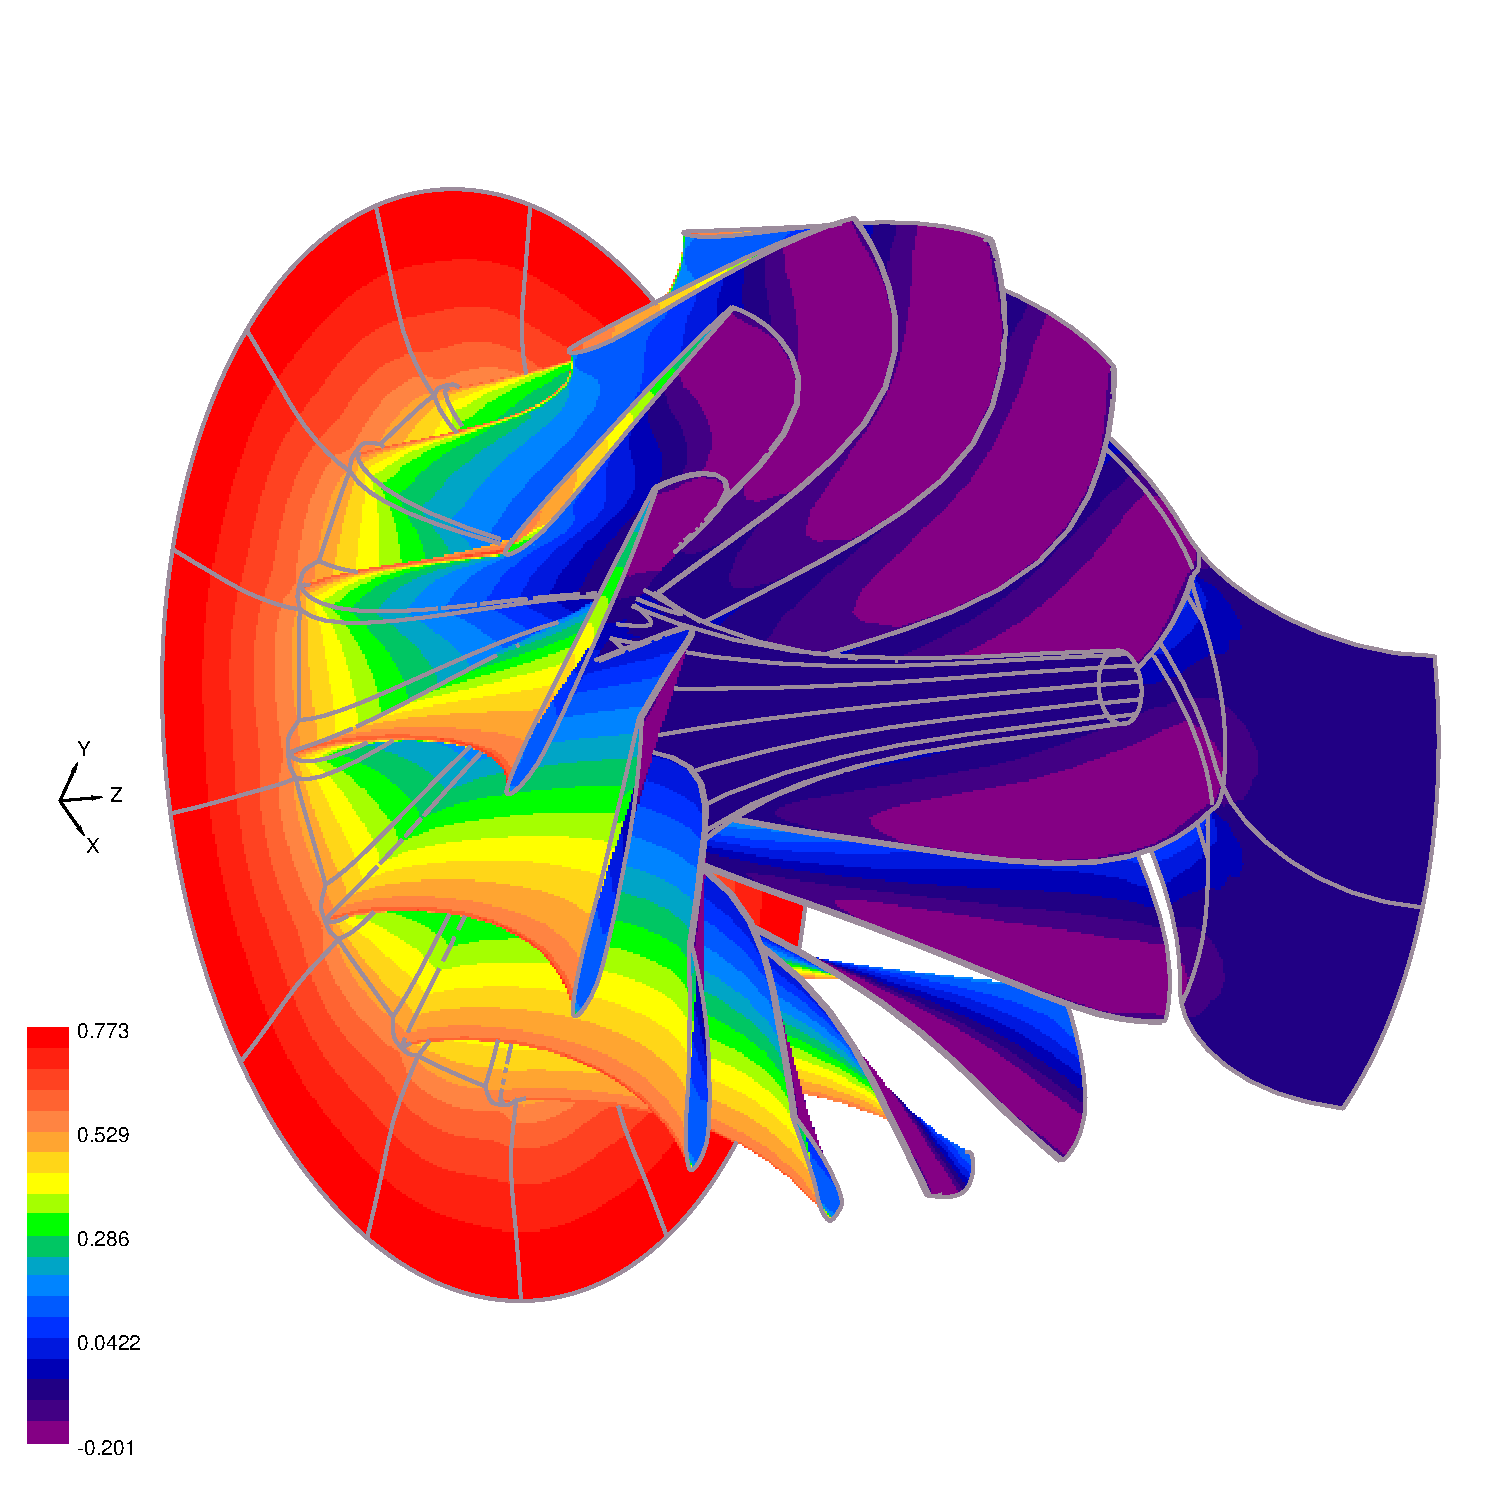
\includegraphics{Cavitation.eps}}
%\end{minipage}
%\caption{Left; $\sigma_{histogram}$ is equal to the $\sigma$ value for which a specific percentage of the blades surface "A" has lower pressure values than $p_{Hist}$, here A is set equal to $0.2\%$ of the blades surface, A is the blade surface that corresponds to the gray area here; Francis runner $\sigma$ contour plot. }
%\label{design-cav}
%\end{figure}


\subsection{Outlet velocity profiles}
Coupling the turbine runner with a pre-existing draft-tube is controlled via the outlet velocity profile metrics. This requires the definition of a target distribution and, thus, the corresponding metric stands for the deviation of the acquired distribution from the target one (fig.\ref{design-obj2}). To perform optimally, a given draft-tube must have, at its inlet, a specific mass-flow ($C_m=\frac{c_m}{\sqrt{2gH}}$) and  specific swirl ($C_u=\frac{c_u}{\sqrt{2gH}}$) span-wise distribution where, $c_m$ and $c_u$ are the meridional and circumferential components of the flow velocity respectively.

%\begin{eqnarray}
%		C_m=\frac{c_m}{\sqrt{2gH}}
%\label{Cavi4}
%\end{eqnarray}
%and 
%\begin{eqnarray}
%		C_u=\frac{c_u}{\sqrt{2gH}}
%\label{Cavi4}
%\end{eqnarray}
%where $c_m$ and $c_u$ are the meridional and circumferential components of the flow velocity respectively.

Therefore the  ``outlet velocity quality" metric is defined as minimization of the deviation between the acquired distributions and the corresponding target. 

\begin{figure}[h!]
\begin{minipage}[b]{1\linewidth}
 \centering
 \resizebox*{10.0cm}{!}{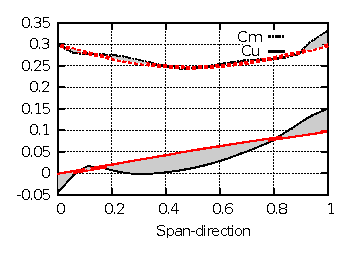
\includegraphics{OUTLET.eps}}
\end{minipage}
\caption{Outlet velocity distributions (thin lines) and the draft-tube specific target distributions (thick lines). $C_m$ is depicted with dashed line and $C_u$ with a solid one. The "outlet quality" optimization objective, deviation between distributions and targets, is depicted hear as the gray area.}
\label{design-obj2}
\end{figure}

%Even though allowing swirl at the runners outlet, as it is shown in figure \ref{design-obj2}, reduces its efficiency as an isolated part, it is needed to ensure the absence of flow detachment in the draft tube witch if happened would result in a dramatic drop in efficiency of the turbine as a hole.  



\subsection{Blade loading quality metric}
Loading quality refers to the way load (eq. \ref{load}) is destributed along the runner blade surface. Constant load along the blade, in chordwise direction, is desirable (fig.\ref{design-obj}) and is linked both to hydraulic quality and good structural behaviour. Load, at each blade position, is defined as the integral of pressure coefficient deference $(C_p^{PS}-C_p^{SS})$ over the blade surface. 
%Chrodwise distribution of load for a given profile can be calculated via splitting the chord in $n$ equal segments of length $d_x$ then the load for every position of the chord can be calculated as; (fig.\ref{design-obj})     

\begin{align} 
   Load(x)=\int (C_p^{PS}(x)-C_p^{SS}(x))) dx 
\label{load}
\end{align}

%where,
%\begin{eqnarray}
%		C_p=\frac{P_{tot,exit}-P}{\rho_{L}gH}
%\label{Cpdef}
%\end{eqnarray}
%The $C_p$ definition used herein is equivalent with the $\sigma$ definition, see above, and will be used both to track Load quality and cavitation danger.  
  

\begin{figure}[h!]
\begin{minipage}[b]{0.5\linewidth}
 \centering
 \resizebox*{7.0cm}{!}{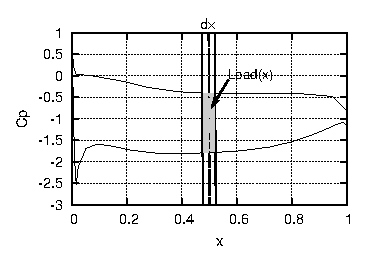
\includegraphics{CP.eps}}
\end{minipage}
\begin{minipage}[b]{0.5\linewidth}
 \centering
 \resizebox*{7.0cm}{!}{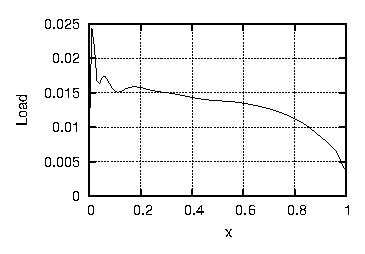
\includegraphics{Load.eps}}
\end{minipage}
\caption{Left: Load definition . Right: Chordwise load distributions of the profile demonstrated left, based on the load definition.}
\label{design-obj}
\end{figure}

Since constant load along the blade, in the chordwise direction, is desirable, optimization should aim at the minimization of standard deviation of the load along the blade surface . 


\subsection{Pumping surface metric}
In case of non-regulated hydraulic turbines, such as Hydromatrix$\circledR$ (section \ref{Matrix-case}), an extra quality metric, concerning their operation at part load, must be introduced.      

In non-regulated machines neither the stator, nor the rotor blades can be rotated so to adjust incoming/outgoing flow directions. During part load operation, this leads to flows with negative incidence angles (meet the blade at the suction side) (fig.\ref{design-pumpS}) thus creating a region where suction side has higher pressures than pressure side. This part of the blade is operating as a pump and, in a well performing turbine, this must be minimum. 

\begin{figure}[h!]
\begin{minipage}[b]{1\linewidth}
 \centering
 \resizebox*{10.0cm}{!}{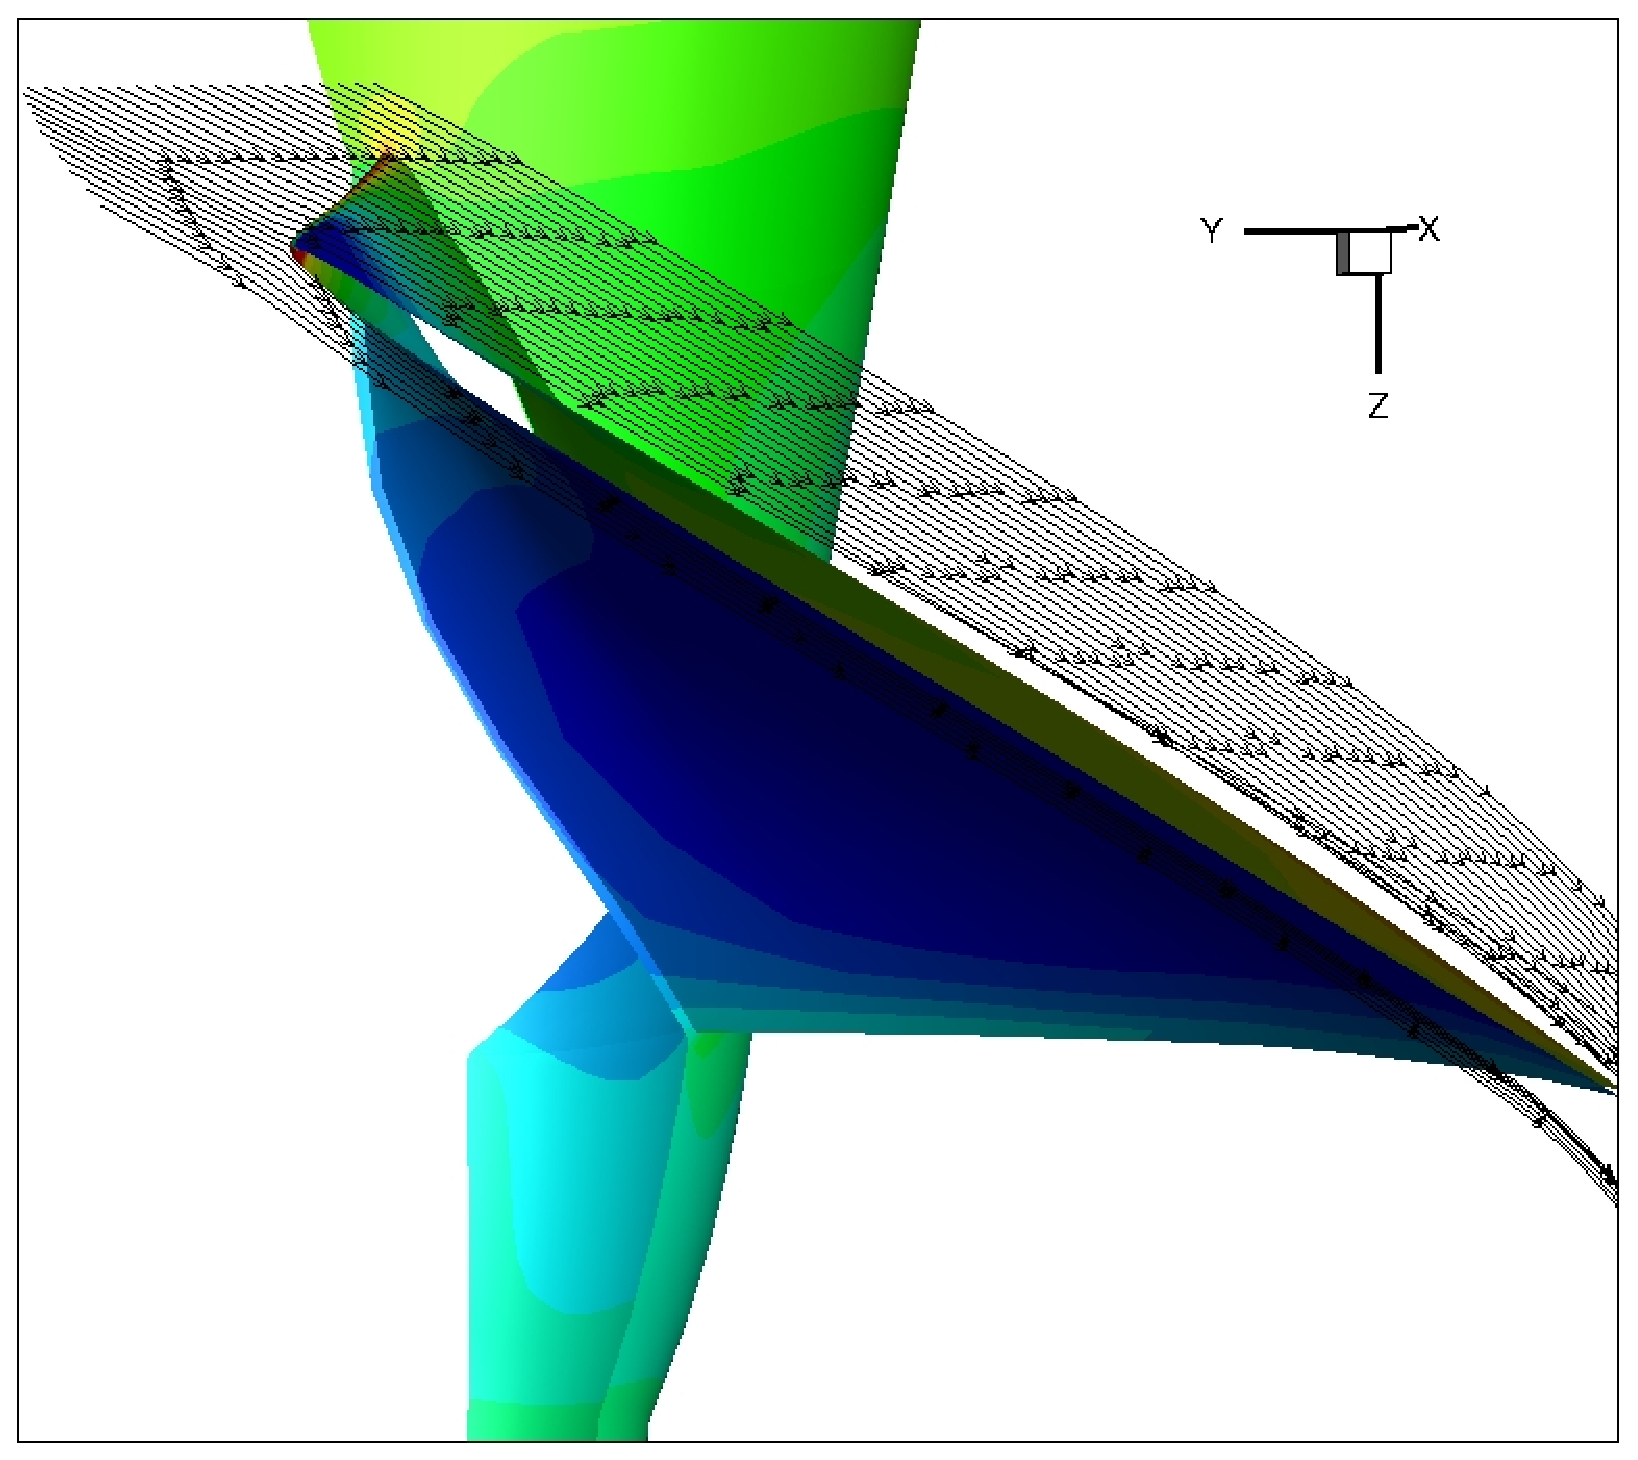
\includegraphics{PartLoad.eps}}
\end{minipage}
\caption{Pressure contour, along with streamlines near the shroud region, at part load operation of a non regulated hydraulic turbine. Water flow near the shroud region has negative incidence angle and, therefore the aforementioned pumping surface is formed. This surface needs to be minimized. }
\label{design-pumpS}
\end{figure}

In figure \ref{design-pumpS}, one may observe the flow streamlines, at the near shroud region, and how they meet the blade at the suction side (bottom the this plot). This causes both a high pressure region at the suction side, due to the stagnation point at the point where the flow meets the blade,  and a low pressure region on the pressure side (top here) due to high flow speeds.        

\begin{figure}[h!]
\begin{minipage}[b]{1\linewidth}
 \centering
 \resizebox*{10.0cm}{!}{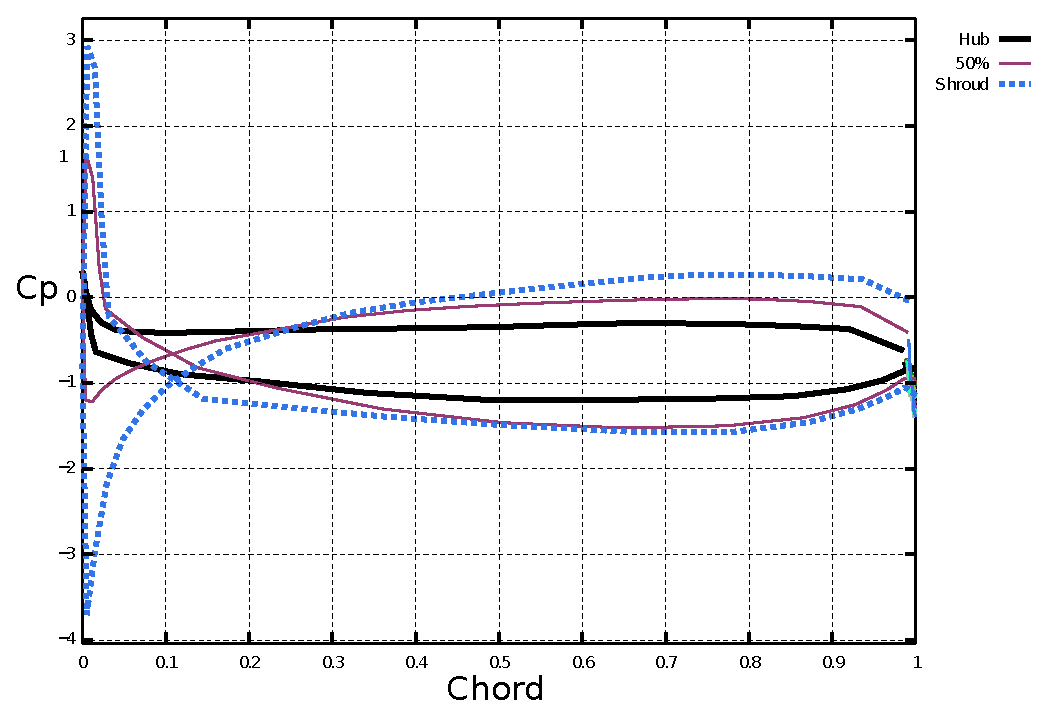
\includegraphics{pumps.eps}}
\end{minipage}
\caption{Pressure coefficient ($C_p$) distribution along the blade chordwise direction at part load operation of a non-regulated hydraulic turbine at three spanwise locations: hub, mid-span and shroud. The pumping area corresponds to the first 10\% of the chord at mid-span and shroud locations}
\label{design-pumpS2}
\end{figure}

The partial pumping operation phenomenon can also be observed by the pressure coefficient ($C_p$) plots, see figure \ref{design-pumpS2}. The near hub $C_p$ distribution (thick continuous line) exhibits no such phenomenon, as expected.  The near shroud $C_p$ distribution (thick dashed line) though suffers from partial pumping operation. The near LE region of the shroud $C_p$ distribution exhibits the so called "crossed" distribution which denotes that the pressure at the pressure side of the blade is lower than that of the suction side. The thin continues line is the mid-span $C_p$ distribution and it also suffers from pumping operation, without however being as severe as close to shroud.        
\FloatBarrier
\section{Optimization of a Francis Turbine} % top level followed by section, subsection
The design-optimization of a Francis turbine runner is presented in this section. This case, due to the high number of design variables used to parameterize the candidate geometries, will be used to demonstrate the merits of the KBD method. 
\label{Francis-runner}
\subsection{Francis Turbine}
Nowadays, Francis turbines are the most frequently used water turbines since they can operate in a considerable part of the head-discharge diagram (fig.\ref{range}). Francis is a reaction type water turbine which was named after its developer James B. Francis. 

\begin{figure}[h!]
\centering
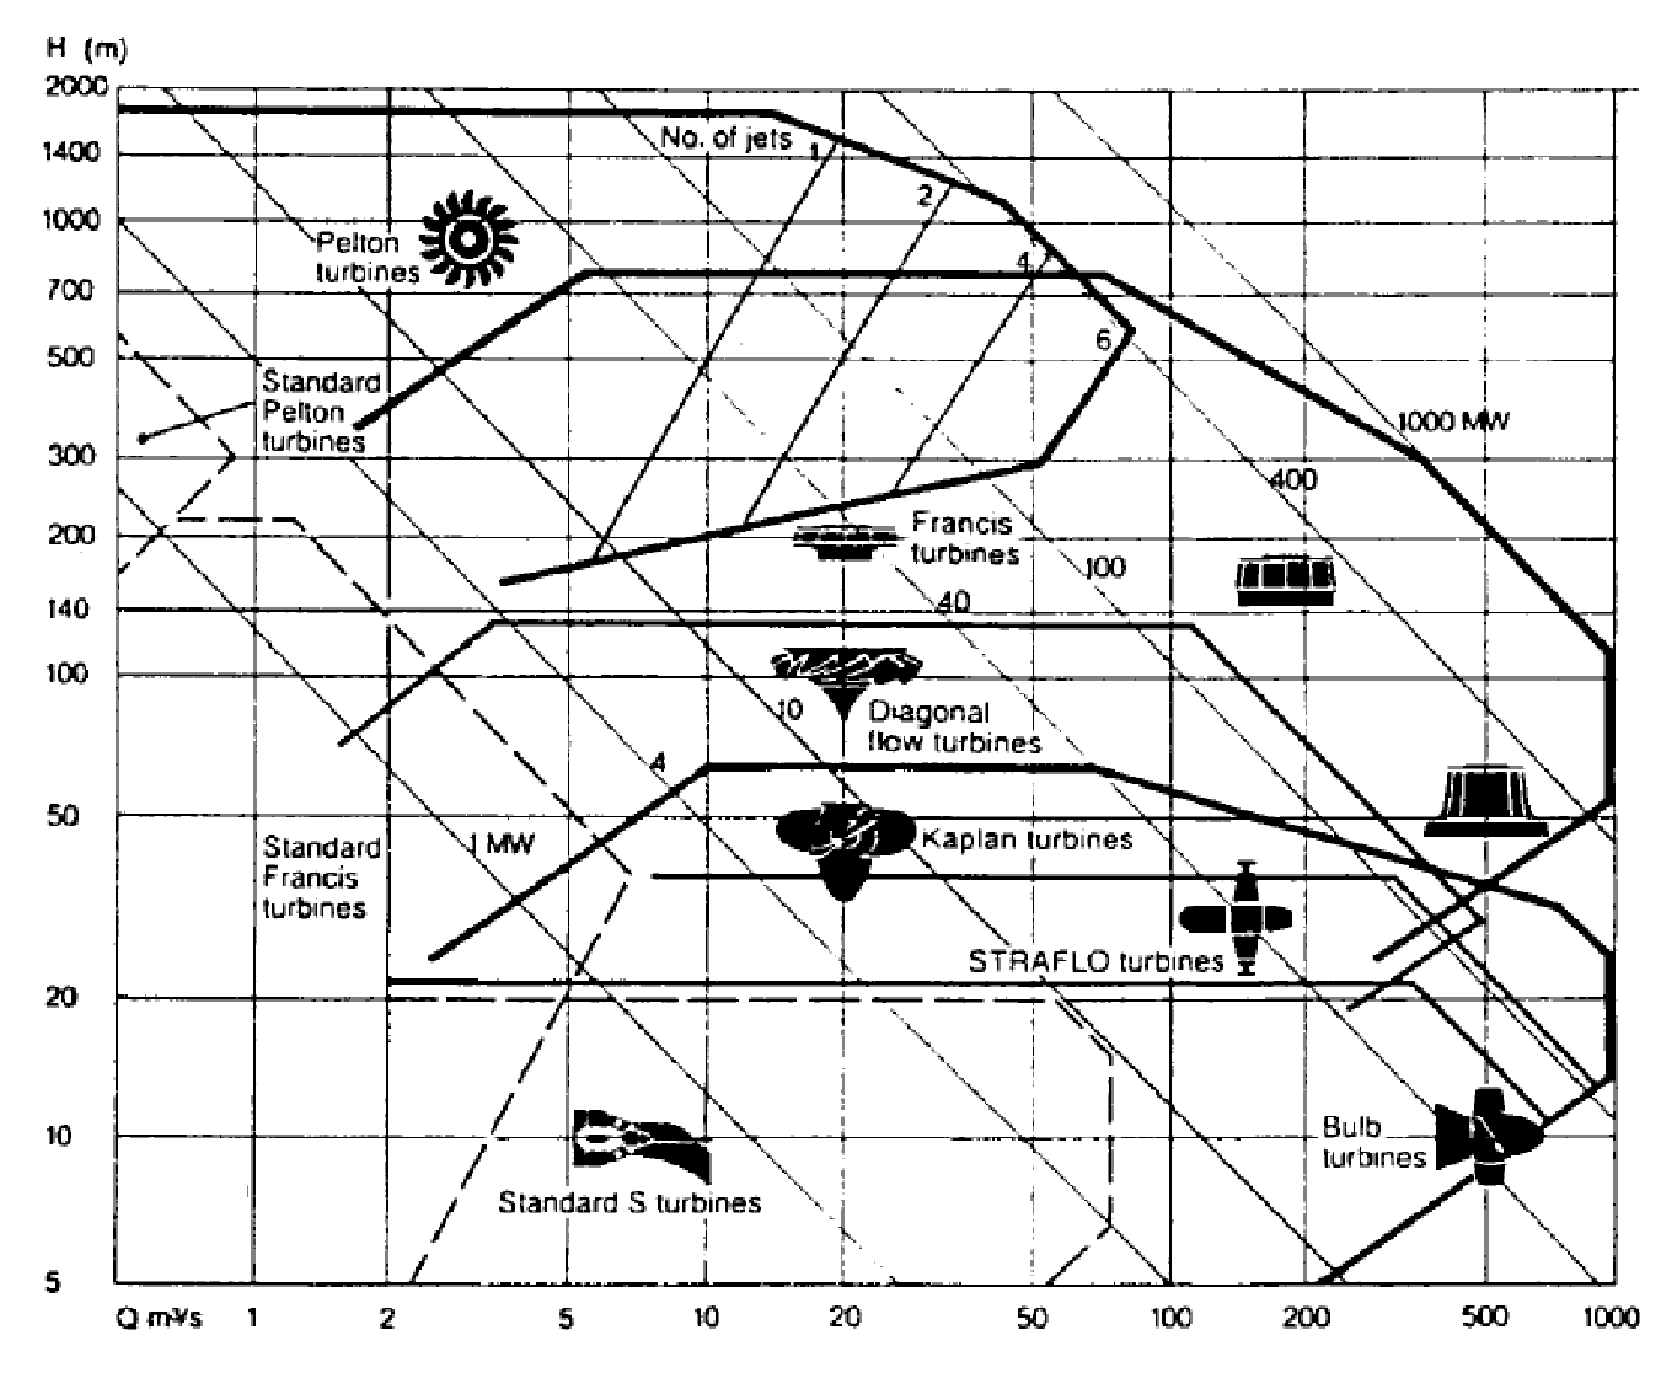
\includegraphics[width=140mm]{range2.eps} 
\caption{Application of different turbine types \cite{papanto}.}
\label{range}
\end{figure}

A typical Francis turbine consists of four different parts (fig.\ref{francis1}). The spiral casing together with the stay-vanes are designed to provide uniform water intake along the entire circumference of the wicket-gates inlet. The wicket-gates (or guide-vanes) are adjustable blades allowing efficient turbine operation for a range of water flow conditions. The runner, which is the rotating part aims, at harnessing the hydraulic energy. Finally, the draft-tube is used to transform the outlet kinetic energy into head.

\begin{figure}[h!]
\centering
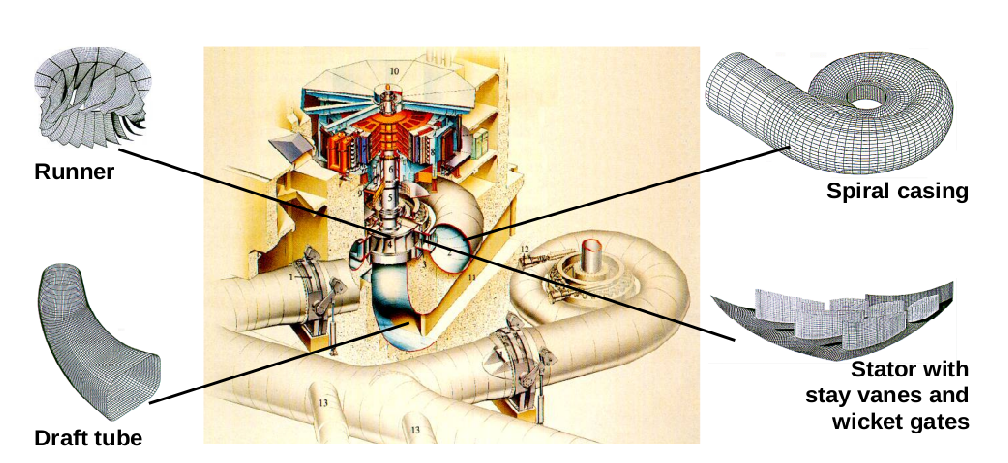
\includegraphics[width=150mm]{francis1.eps} 
\caption{Francis turbine and its consisting parts \cite{andritz}.}
\label{francis1}
\end{figure}

\subsection{Case presentation}
From the industrial point of view, the design problem in hand is referred to as a modernization/rehabilitation project, since it mainly aims at upgrading the runner (fig.\ref{design-parameterization}) for use in a pre-existing power plant. Modernization/rehabilitation projects are fairly common world-wide and, especially in Europe where almost all large-hydro locations are already tapped and a lot of them are ``aged''. Typical reasons for modernization/rehabilitation project are;
\begin{itemize}
\item[\textbf{(a)}] to increase the reliability and availability of the power plant; 
\item[\textbf{(b)}] to extent its life and restore its performance; 
\item[\textbf{(c)}] to improve its performance, including;
\begin{itemize}
	\item efficiency and/or power;
    \item reduction of cavitation erosion and;
	\item enlargement of the operating range;
\end{itemize}
\item[\textbf{(d)}] to improve the plant safety;
\item[\textbf{(e)}] to resolve environmental, social or regulatory issues;
\item[\textbf{(f)}] to reduce the maintenance or operating cost;
\item[\textbf{(g)}] to take into account other considerations, such as;
\begin{itemize}
	\item modified governmental regulations;
	\item political criteria;
	\item modified hydrology conditions or;
	\item modified market conditions;
\end{itemize}
\end{itemize}

In modernization/rehabilitation projects, the designer must ensure that the newly designed runner fits perfectly into the pre-existing structure by respecting both geometric and hydraulic-behaviour constraints. Geometric constraints are mostly related with the inlet-outlet diameters and the hub-shroud meridional contour. On the other hand, hydraulic behaviour enforces given inlet conditions and introduces a new objective, apart from efficiency and cavitation,  which is associated with the draft-tube coupling since, at the outlet, of the newly designed runner meets the draft-tube inlet and any given draft-tube works optimally for a specific inlet velocity profiles.      
  
\begin{figure}[h!]
\begin{minipage}[b]{1\linewidth}
 \centering
 \resizebox*{7cm}{!}{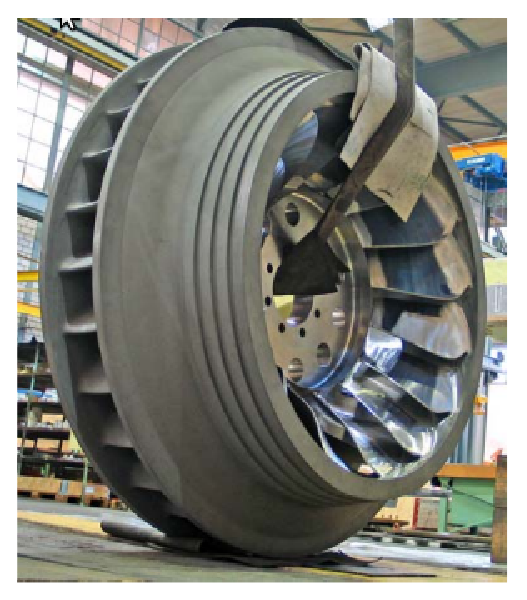
\includegraphics{francis2.eps}}
\end{minipage}
%\begin{minipage}[b]{0.5\linewidth}
% \centering
% \resizebox*{7.5cm}{!}{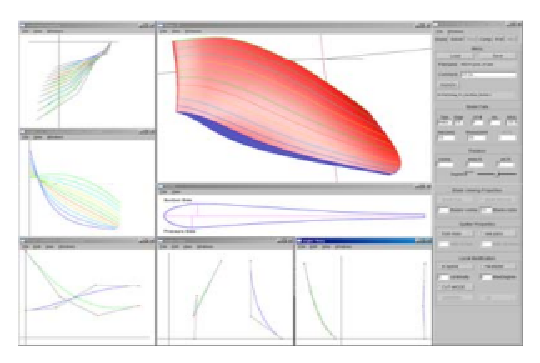
\includegraphics{francis3.eps}}
%\end{minipage}
\caption{Optimization of a Francis Turbine: View of a Francis runner similar to the one designed herein \cite{andritz}. }%Right; demonstration of Francis runner parameterization}
\label{design-parameterization}
\end{figure}

%\subsubsection{Case formulation}
%Herein the case formulation that transforms the above design case into a basic optimization problem will be presented. Given that the optimization problem definition is (cite EA chapter);
%\begin{align} 
%   &min ~ F(x)=(f_1(x),f_1(x),...,f_M(x))\in \Re^{M} \nonumber \\
%   &\mbox{subject to} ~ c_k(x)\leq d_k ~ k =1,K
%\label{Optim}
%\end{align}
%,where $x\in X \!\leq\! \Re^{N}$ is the design vector and $X$ the design space, $c(x)$ the constraints vector and $F(x)$ the objectives vector.

\subsubsection{Design parameterization}
The design variables and their corresponding ranges are picked from the set specified in section \ref{Paramt} through a user friendly graphical interface integrated in the parameterization tool \cite{dipl_livia,dipl_simon}.  For the case in hand, the design vector consists of $336$ free design variables as in table \ref{design_vars}.


%\begin{figure}[h!]
%\begin{minipage}[b]{1\linewidth}
% \centering
% \resizebox*{7cm}{!}{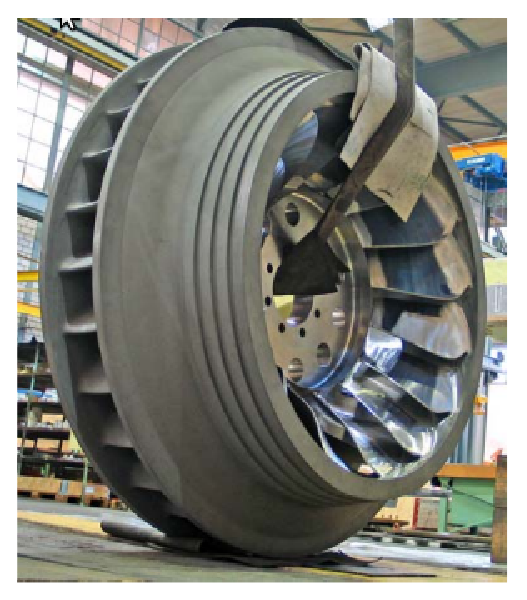
\includegraphics{francis2.eps}}
%\end{minipage}
%\begin{minipage}[b]{1\linewidth}
% \centering
% \resizebox*{14cm}{!}{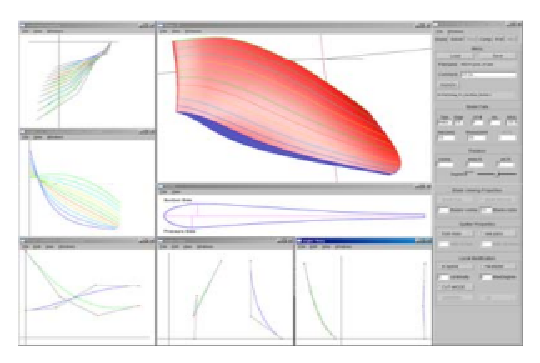
\includegraphics{francis3.eps}}
%\end{minipage}
%\caption{Optimization of a Francis Turbine: Graphical interface integrated in the parameterization tool.}
%\label{design-parameterization}
%\end{figure}


\begin{table}[h!]
\begin{center}
\begin{tabular}{ |c|l| }
\hline

Number of              & used to parameterize the:\\
design variables       & \\
\hline
6 & spanwise distributions of $\theta_{LE}$\\
\hline
6 & spanwise distributions of $\theta_{TE}$\\
\hline
6 & spanwise distributions of $\beta_{LE}$\\
\hline
6 & spanwise distributions of $\beta_{TE}$\\
\hline
6 & spanwise distributions of $\zeta_{LE}$\\
\hline
6 & spanwise distributions of $\zeta_{TE}$\\
\hline
6 & spanwise thickness distributions for PS \\
\hline
6 & spanwise thickness distributions for SS\\
\hline
8 & LE projection on the meridional plane\\
\hline
8 & TE projection on the meridional plane\\
\hline
4 & shroud generatrix (on the meridional plane) \\
\hline
4 & hub generatrix (on the meridional plane)\\
\hline
$12 \times 11$ & water-foil profiles for the PS (11 profiles)\\
\hline
$12 \times 11$ & water-foil profiles for the SS (11 profiles)\\
\hline
\hline
336 & Design variables, in total \\
\hline   
\end{tabular}
\caption{
The design variables used to parameterize the Francis runner.}
\label{design_vars}
\end{center}
\end{table}

%\begin{figure}[h!]
%\begin{minipage}[b]{1\linewidth}
% \centering
% \resizebox*{13cm}{!}{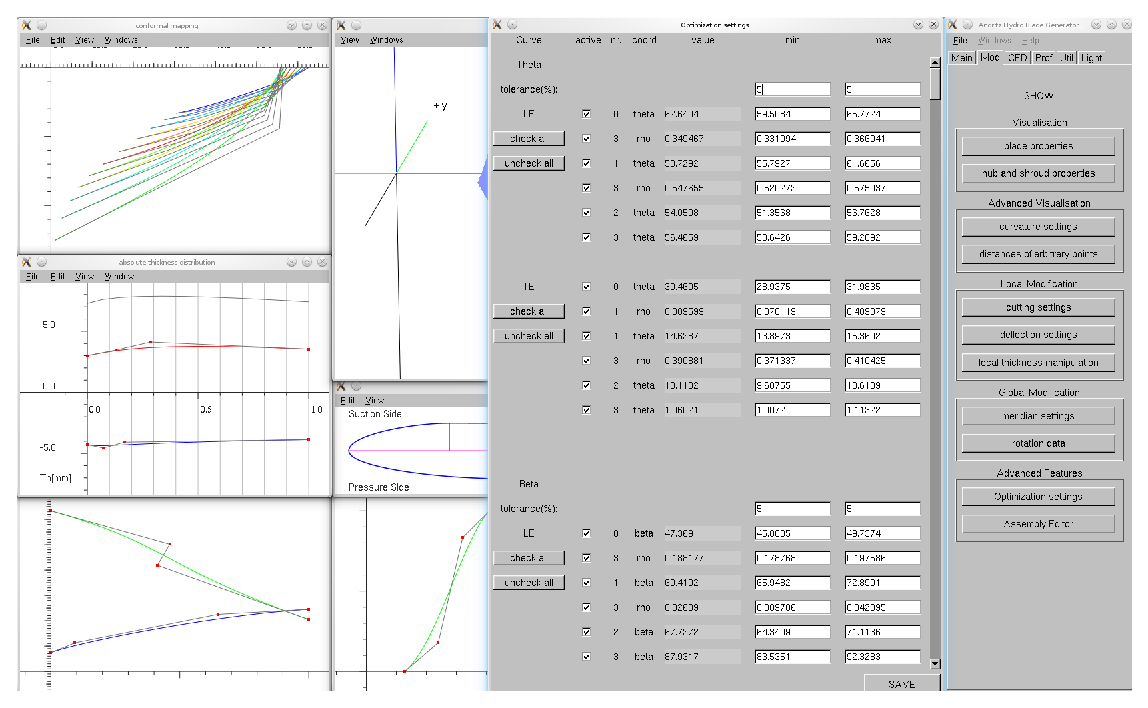
\includegraphics{pic2.eps}}
%\end{minipage}
%\caption{Optimization of a Francis Turbine: Graphical interface integrated in the parameterization tool.}
%\label{design-parameterization2}
%\end{figure}

\subsubsection{Objectives and Constraints}
The objectives vector consist of two objectives, which correspond to the outlet velocity profile metric ($M_1$) and the blade loading quality one ($M_2$). To define $M_1$, the user defined target profiles as they are shown in figure \ref{design-obj-tar}. 



\begin{figure}[h!]
\begin{minipage}[b]{1\linewidth}
 \centering
 \resizebox*{10.0cm}{!}{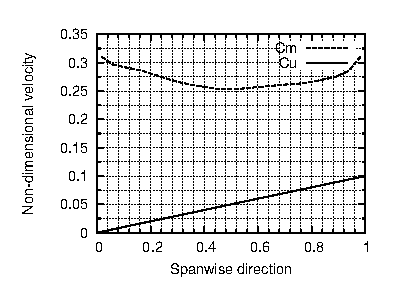
\includegraphics{Target.eps}}
\end{minipage}
\caption{Optimization of a Francis Turbine: Target nondimensional velocity profile distributions at the runner-outlet.}
\label{design-obj-tar}
\end{figure}


To ensure performance stability, the runner to be designed is desirable to yield optimal performance at three operating points, the best efficiency (BE) point, the part load (PL) and full load (FL) ones. %(best efficiency point H=36m, part load H=30m and full load H = 43.5m). 
The three-operating-point design is handled as an optimization problem with two objectives, where the value of each objective function is computed for each operating point separately (equation \ref{ObjFrancis}) and, then, the “overall” value $f_i$ is set equal to the weighted sum (equation \ref{ObjFrancis2}) of the corresponding values for the three operating points. (table. \ref{op-weights}) 


\begin{eqnarray}
   f_1^i=M_1^i ~~~\&~~~ f_2^i=M_2^i 
   \label{ObjFrancis} 
\end{eqnarray}
where the superscript $i=1,2,3$ denotes the operating point.

\begin{eqnarray}
   f_1=\sum^3_{i=1}w_if_1^i ~~~\&~~~ f_2=\sum^3_{i=1}w_if_2^i 
   \label{ObjFrancis2} 
\end{eqnarray}
where $w_i$ the weight per operating point (table \ref{op-weights}).


\begin{table}[h!]
\begin{center}
\begin{tabular}{ |c|l| }
\hline
Operating point& Weight $(w_i)$\\
\hline
Best Efficiency (BE), $i=1$ & 1.0\\
\hline
Part Load (PL), $i=2$ & 0.3\\
\hline
Full Load (FL), $i=3$ & 0.3\\
\hline
\end{tabular}
\caption{Optimization of a Francis Turbine: Operating point weights.}
\label{op-weights}
\end{center}
\end{table}


For each operating point, two constraints are set (table \ref{Cons}). The first is related to the cavitation safety and the second aims at ensuring that the turbine is operating at the desired point. The cavitation constraint is based on the $\sigma_{Hist}$ method as presented in section \ref{cav.metric}. Operating point control is carried out by imposing a constraint on the maximum distance from the desired operating point. Here, given that the massflow is used to define the boundary conditions, the operating point is controlled via a constraint imposed onto the hydraulic height.     


\begin{eqnarray}
   \Delta H=\frac{H_{computed}-H_{desirable}}{H_{desirable}} 
   \label{ConstFrancis} 
\end{eqnarray}
where $H_{desirable}$ the desirable $H$ specified by the desirable operating point.

\begin{table}[h!]
\begin{center}
\begin{tabular}{ |c|c|c| }
\hline
Operating point & $\sigma_i^{Hist}<\sigma$ & Hydraulic hight\\
\hline
BE & $\sigma_i^{Hist}<0.2$ & $|\Delta H^i|<1.5\%$\\
\hline
PL       & $\sigma_i^{Hist}<0.2$ & $|\Delta H^i|<5\%$\\
\hline
FL       & $\sigma_i^{Hist}<0.2$ & $|\Delta H^i|<5\%$\\
\hline
\end{tabular}
\caption{Optimization of a Francis Turbine: Constraints per operating point.}
\label{Cons}
\end{center}
\end{table}


%\begin{figure}[h!]
%\begin{minipage}[b]{0.5\linewidth}
% \centering
% \resizebox*{7.0cm}{!}{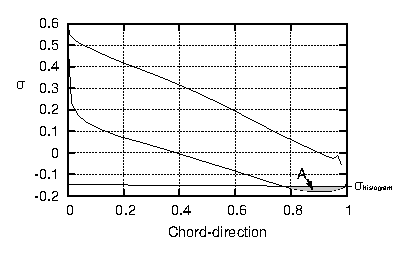
\includegraphics{sigma.eps}}
%\end{minipage}
%\begin{minipage}[b]{1\linewidth}
% \centering
% \resizebox*{10.0cm}{!}{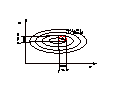
\includegraphics{con1.eps}}
%\end{minipage}
%\caption{Optimization of a Francis Turbine: Maximum distance from %operating point equals to $\pm2\%$.}
%\label{design-obj3}
%\end{figure}

\subsection{Results}
As mentioned above, this case is used to demonstrate the KBD method, proposed in this thesis, in a real industrial case. Therefore, two optimization procedures are tried; one by using the conventional EA since the large number of design variables makes the use of metamodels (as in standard MAEA) inefficient; and the MAEA(KBD) method proposed herein.

\subsubsection{Archived designs}
Three archived designs were available (fig.\ref{design-bases}). These designs were developed to perform optimally in operating points close to those set for the desired blade. The criteria used to estimate this vicinity were the nondimensional specific speed $N_{ED}$ and specific massflow $Q_{ED}$ \footnote{$N_{ED}$ and $Q_{ED}$ are dimensionless terms based on energy (E=1) and diameter (D=1) that characterize machine operation.} as defined in equation \ref{undimFrancis}. 

\begin{eqnarray}
   N_{ED}=\frac{n}{60}\frac{D}{\sqrt{gH}}, ~~~~~~ Q_{ED}=\frac{Q}{D^2 \sqrt{gH}}
   \label{undimFrancis} 
\end{eqnarray}

%Since those design were fitted with their own, power plan specific, hub and shroud contours and given that during the modernization/rehabilitation project in hand. Those contours was asked to remain similar to the initial blade, some modifications were required in order to transform the archived designs into compatible with the required hub and shroud contours limitations. These modifications were restricted to simple stretching and pruning, something that requires practically zero time for the designer. However, as will be shown later in this section, this leads to designs with questionable quality. Nevertheless, this designs, with out any further hand-made refinements, are sufficient to be used as basis vectors in the KBD method.                           

\begin{figure}[h!]
\begin{minipage}[b]{1\linewidth}
 \centering
 \resizebox*{10.0cm}{!}{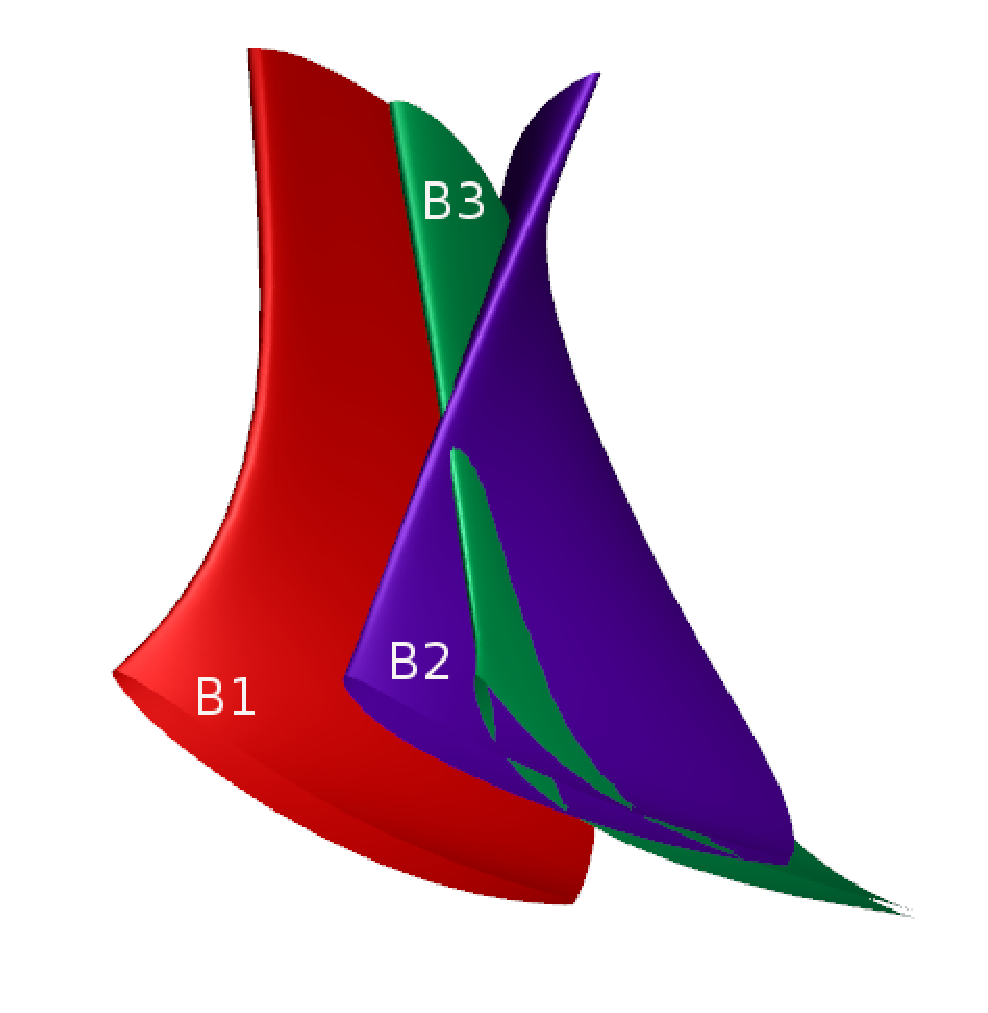
\includegraphics{Francis_bases.eps}}
\end{minipage}
\caption{Optimization of a Francis Turbine: The three archived geometries used for this case.}
\label{design-bases}
\end{figure}

The archived designs to be used as basis vectors for this case are re-evaluated at the desirable operating points and their quality metrics are summarized in table \ref{reuse}.

\begin{table}[h!]
\begin{center}
\begin{tabular}{ |c|c|c|c|c|c| }
\hline
Archived & OP & $M_1$ & $M_2$  & $\sigma_i^{Hist}$ & $|\Delta H|$\\
Design &&&&&\\
\hline
 & BE & $0.472$ & $0.538$ & $0.21 > 0.2$ * & $ 5\% >1.5\%$ * \\
B1 & PL & $0.552$ & $0.824$ & $0.23 > 0.2$ * & $ 3.6\% <5\%$ \\
& FL & $0.408$ & $0.594$ & $0.2 = 0.2$  & $ 5.7\% >5\%$ * \\
\hline
\hline
& BE & $0.563$ & $0.922$ & $0.22 > 0.2$ * & $ 3.8\% >1.5\%$ * \\
B2 & PL & $0.534$ & $0.888$ & $0.24 > 0.2$ * & $ 2.6\% <5\%$  \\
& FL & $0.522$ & $1.178$ & $0.22 > 0.2$ * & $ 4.8\% <5\%$  \\
\hline
\hline
& BE & $0.402$ & $0.663$ & $0.19 < 0.2$  & $ 6.8\% >1.5\%$ * \\
B3 & PL & $0.515$ & $0.808$ & $0.21 > 0.2$ * & $ 6.9\% >5\%$ * \\
& FL & $0.257$ & $0.896$ & $0.18 < 0.2$  & $ 7.1\% >5\%$ * \\
\hline
\end{tabular}
\caption{Optimization of a Francis Turbine: Quality metrics (objectives and constraints) for the 3 archived designs (B1, B2 and B3) for all operating points (BE, PL and FL). An asterisk (*) next to an inequality means that the corresponding constrained is violated}
\label{reuse}
\end{center}
\end{table}

A closer look at B1 reveals the findings tabulated in table \ref{reuse}. For instance, from figure \ref{Francis-B1-BE}, where the  $C_p$ isoareas are plotted over the runner surfaces, areas which are prone to cavitation can readily be identified. From this figure, one may observe the lower limit of $C_p = -0.216$ which advocates the presence of cavitation, since $\sigma_i \approx -C_p=0.216$  . Recall that $\sigma=0.2$ and that $\sigma_i$ must be greater than $\sigma$ for cavitation to appear. A closer look at the $\sigma_i^{Hist}$ value which is equal to $0.21$ confirms that observation. Recall that $\sigma_i^{Hist}$ is a better estimation of $\sigma_i$ than the $-C_p$ one. So, the archived design B1 is suffering from cavitation even at the BE point. Figure \ref{Francis-B1-BE} shows that regions with low $C_p$ along the blade which are prone to cavitation exist at the suction side, near the trailing edge, between mid-span and shroud. The archived design B1 suffers from cavitation at the PL point too and is just marginally safe at the FL operating point (table \ref{reuse}). 

\begin{figure}[h!]
\begin{minipage}[b]{1\linewidth}
 \centering
 \resizebox*{14.0cm}{!}{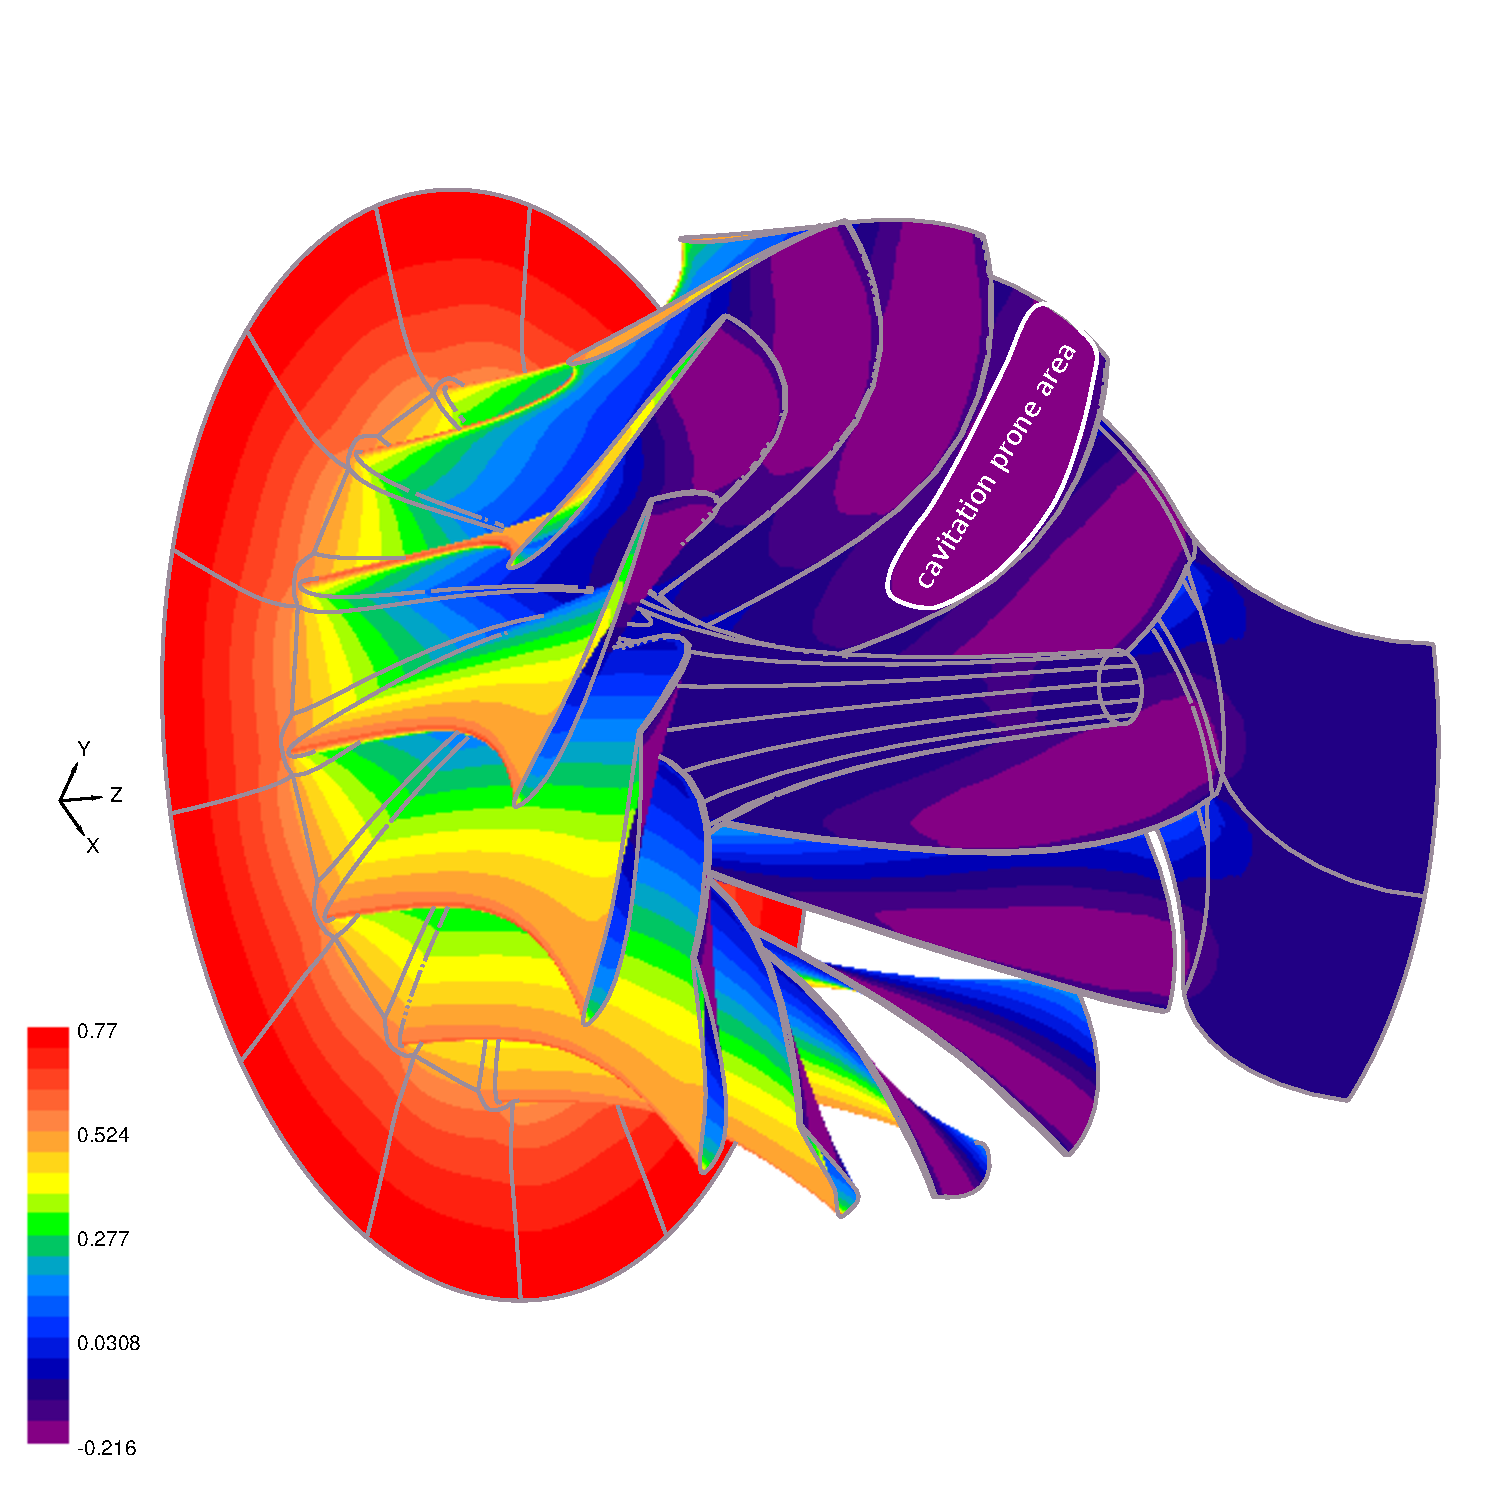
\includegraphics{B1.eps}}
\end{minipage}
\caption{Optimization of a Francis Turbine: $C_p$ isoareas for the archived geometry B1, at the BE operating point. Areas which are prone to cavitation (regions with low $C_p$) can be identified at the suction side, near the trailing edge, between mid-span and shroud.}
\label{Francis-B1-BE}
\end{figure}

Furthermore, regarding the same design  B1, in figure \ref{Francis-B1-OUT} one can observe the noticeable deviation from the desirable outlet $C_m$ and $C_u$ velocity profiles for operating at BE point.  Dashed lines represent $C_m$ and continuous lines $C_u$. For the purpose of comparison, in the same plot, the target distributions are plotted with thicker lines.   

\begin{figure}[h!]
\begin{minipage}[b]{1\linewidth}
 \centering
 \resizebox*{11.0cm}{!}{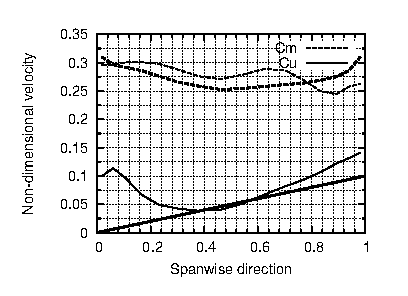
\includegraphics{OUTLET_B1.eps}}
\end{minipage}
\caption{Optimization of a Francis Turbine: $C_m$ and $C_u$ profiles for archived design B1 operating at the BE point. The target distributions are plotted with thicker lines.}
\label{Francis-B1-OUT}
\end{figure}

The loading quality, of B1, can be demonstrated through the $C_p$ chordwise distribution, as defined in eq. \ref{Cpdef}, along the hub, mid-span and shroud (fig. \ref{Francis-B1-LOAD}). Though at the mid-span and the hub relatively good loading behaviour is observed, the blade part which is close to the shroud suffers from important loading differences.      

\begin{figure}[h!]
\begin{minipage}[b]{1\linewidth}
 \centering
 \resizebox*{11.0cm}{!}{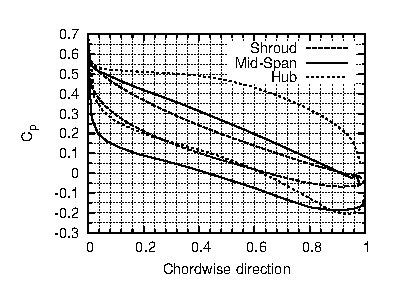
\includegraphics{Load_B1.eps}}
\end{minipage}
\caption{Optimization of a Francis Turbine: $C_p$ profiles hub, mid-span and shroud for archived design B1 for the BE operating point.}
\label{Francis-B1-LOAD}
\end{figure}

\FloatBarrier
Regarding B2, the existing blade suffers from cavitation at all three operating points, see table \ref{reuse}. Figure \ref{Francis-B2-BE} shows the $C_p$ isoareas over the runner blade surface of B2, operating at the BE point. The lower limit of $C_p$, $(C_p\!=\!-0.234)$ denotes that it is likely for cavitationt appear and this is confirmed by the $\sigma_i^{Hist}$ values (table \ref{reuse}). Figure \ref{Francis-B2-BE} shows that cavitation occurs over the suction side near the trailing edge at the near hub region.     


\begin{figure}[h!]
\begin{minipage}[b]{1\linewidth}
 \centering
 \resizebox*{14.0cm}{!}{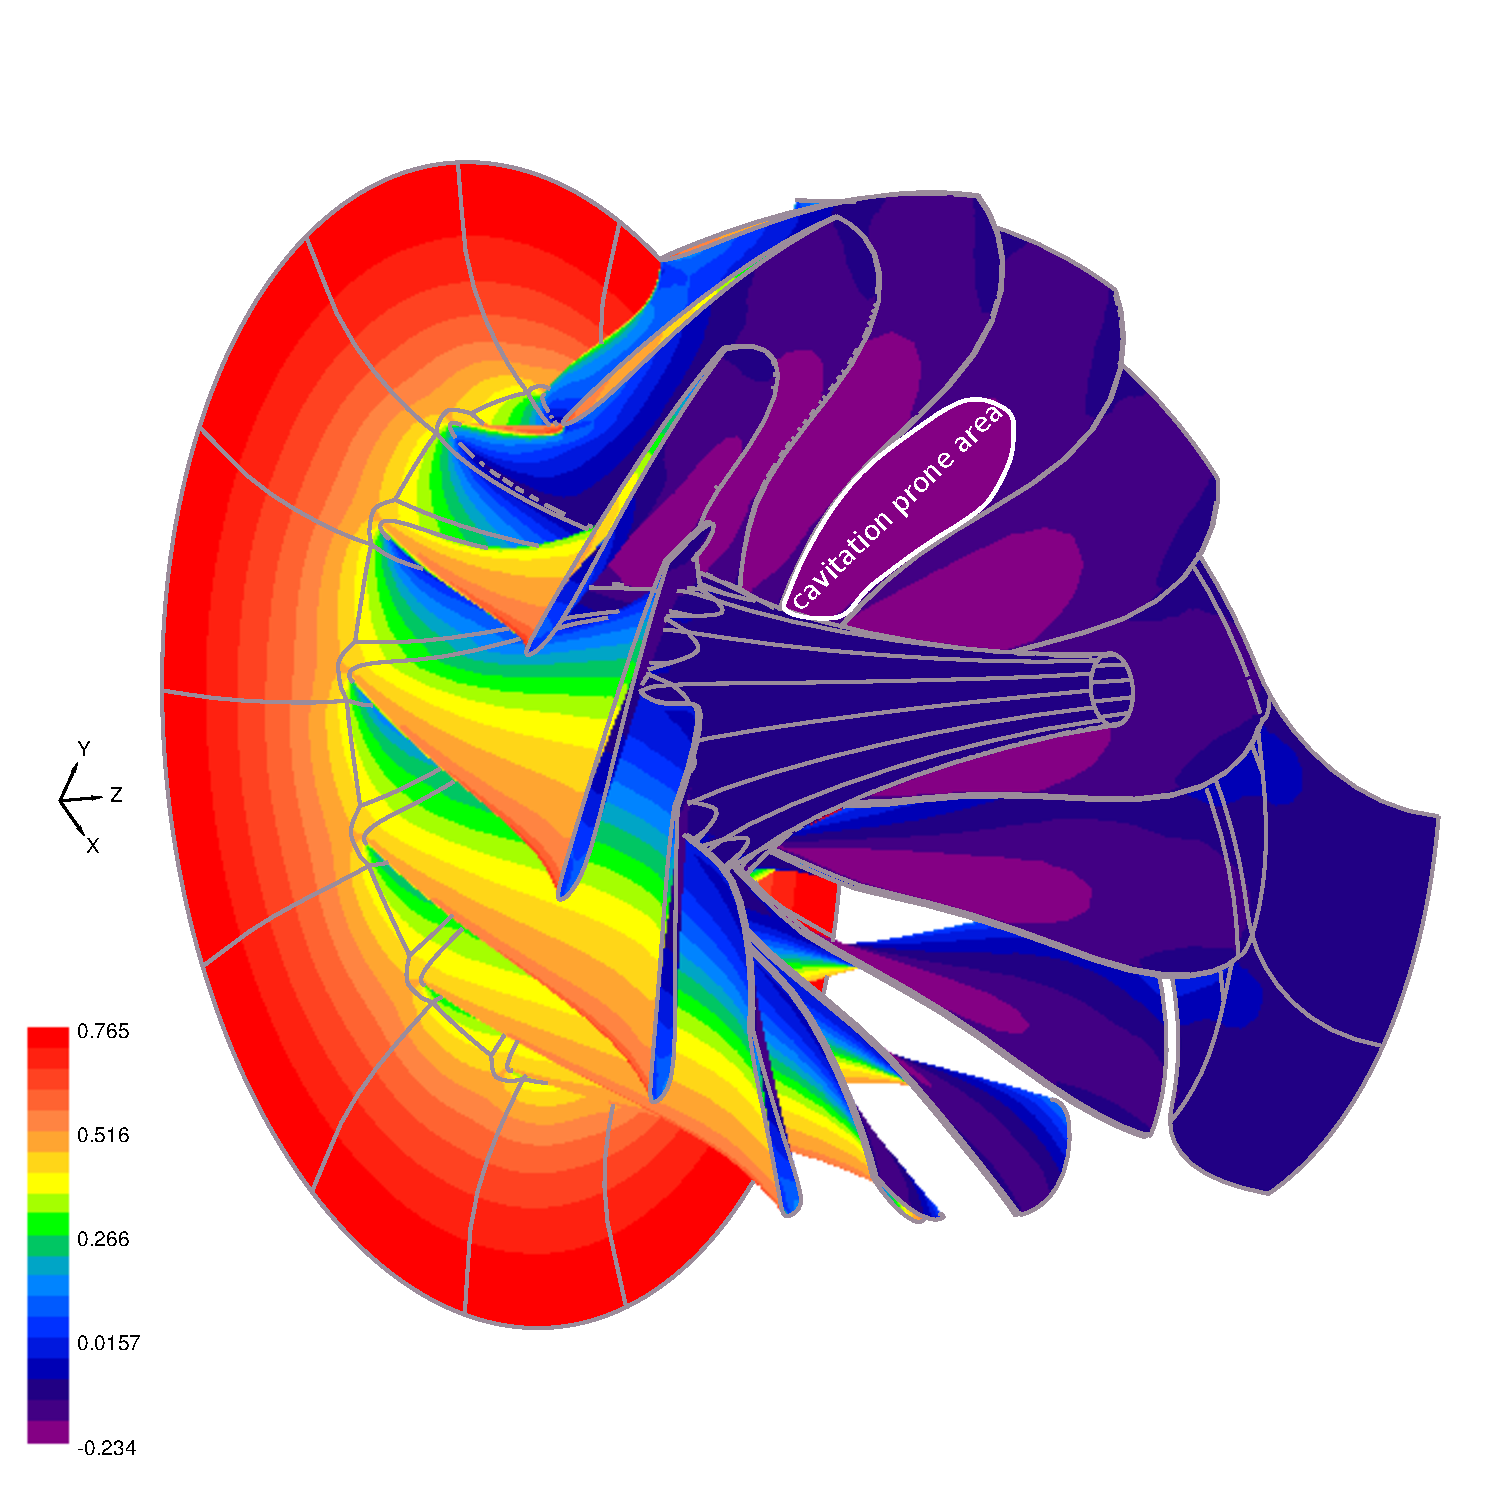
\includegraphics{B2.eps}} %Pics located at /home/stelios/Desktop/BEMPOSTA/MAEA_CBR_case_Bemposta_4/Bases/
\end{minipage}
\caption{Optimization of a Francis Turbine: $C_p$ isoareas for the archived design B2 operating at the BE point. Cavitation occurs on the suction side, near the trailing edge close to the hub.}
\label{Francis-B2-BE}
\end{figure}

The outlet velocity quality is quantified in figure \ref{Francis-B2-OUT}. $C_m$ is far away from the desirable distribution and $C_u$ has high values close to the hub.   

\begin{figure}[h!]
\begin{minipage}[b]{1\linewidth}
 \centering
 \resizebox*{11.0cm}{!}{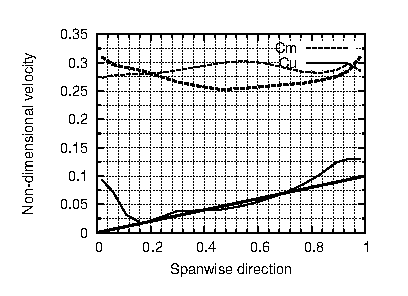
\includegraphics{OUTLET_B2.eps}}
\end{minipage}
\caption{Optimization of a Francis Turbine: $C_m$ and $C_u$ profiles for the archived design B2 at the BE operating point. The target distributions are plotted with thicker lines.}
\label{Francis-B2-OUT}
\end{figure}

From the $C_p$ profiles for the archived design B2 operating at the BE point (fig. \ref{Francis-B2-LOAD}), one may observe the not-satisfactory loading quality, the same information can be obtained from table \ref{reuse}. For the three spanwise positions. there are important load differences along the chord direction. 

\begin{figure}[h!]
\begin{minipage}[b]{1\linewidth}
 \centering
 \resizebox*{11.0cm}{!}{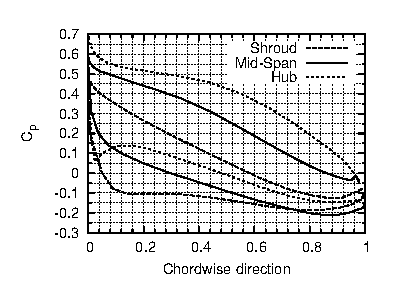
\includegraphics{Load_B2.eps}}
\end{minipage}
\caption{Optimization of a Francis Turbine: $C_p$ profiles at hub, mid-span and shroud for archived design B2 at the BE point.}
\label{Francis-B2-LOAD}
\end{figure}

\FloatBarrier
The archived design B3 is clean from cavitation in all but the PL operating point, see table \ref{reuse}. Figure \ref{Francis-B3-PL} shows the $C_p$ isoareas for  B3 operating at the PL point. The lower $C_p$ value observed, namely $C_p= -0.215$, is a clear indication of the presence of cavitation, as also confirmed by the computed $\sigma_i^{Hist}$ value (table \ref{reuse}). Cavitation is observed at the suction side near the trailing edge.     


\begin{figure}[h!]
\begin{minipage}[b]{1\linewidth}
 \centering
 \resizebox*{14.0cm}{!}{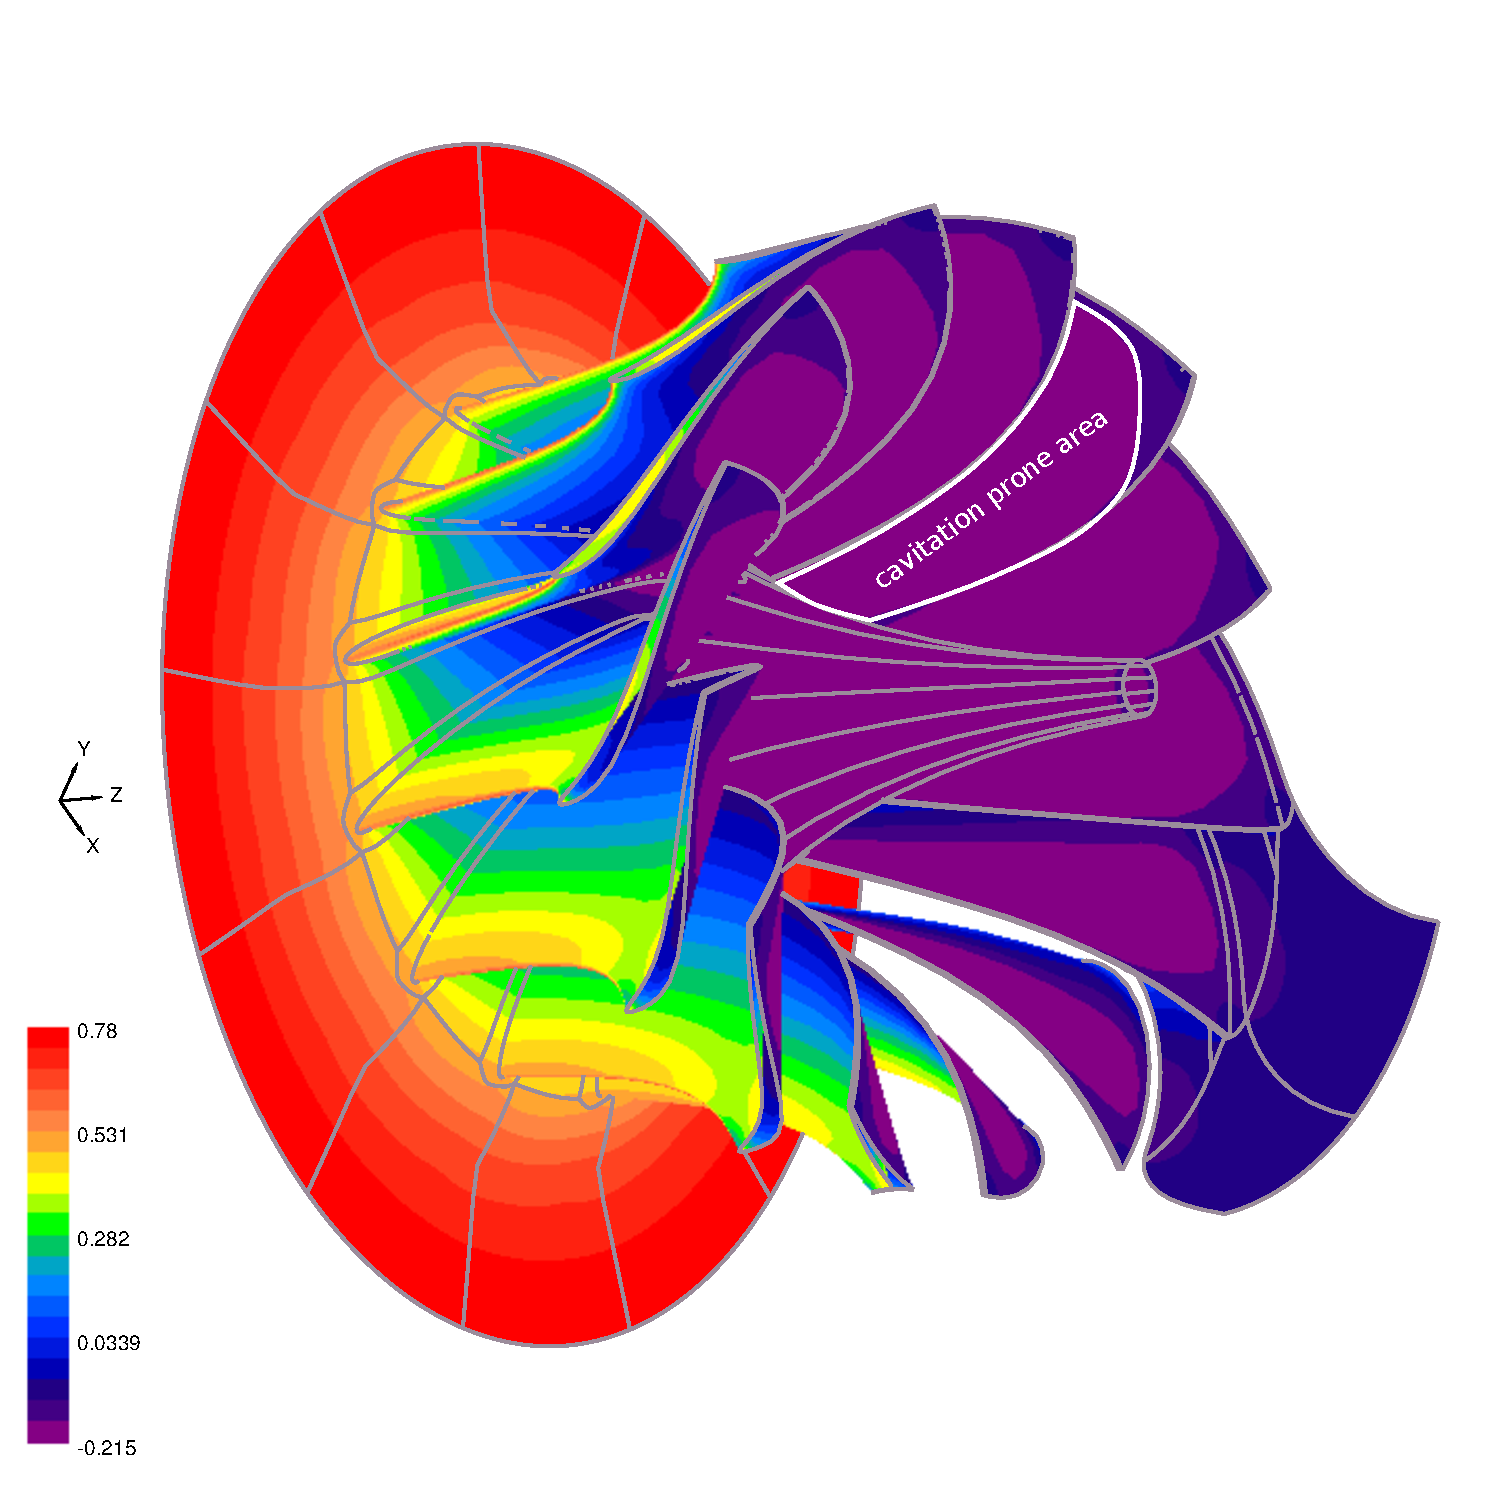
\includegraphics{B3.eps}}
\end{minipage}
\caption{Optimization of a Francis Turbine: $C_p$ isoareas for archived design B3 at PL operating point. Cavitation is observed at the suction side near the trailing edge.}
\label{Francis-B3-PL}
\end{figure}

Regarding the outlet velocity profile quality, figure \ref{Francis-B3-OUT}, both $C_m$  and $C_u$ deviate considerably from the desirable distributions.   

\begin{figure}[h!]
\begin{minipage}[b]{1\linewidth}
 \centering
 \resizebox*{11.0cm}{!}{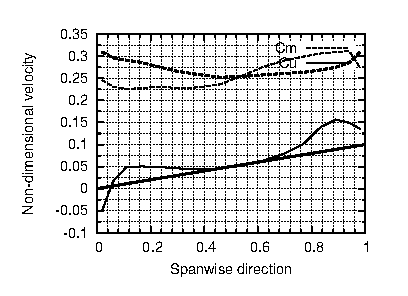
\includegraphics{OUTLET_B3.eps}}
\end{minipage}
\caption{Optimization of a Francis Turbine: $C_m$ and $C_u$ profiles for archived design B3 at the BE operating point. For the purpose of comparison, in the same plot the target distributions are plotted with thicker lines.}
\label{Francis-B3-OUT}
\end{figure}

Loading quality is demonstrated in figure \ref{Francis-B3-LOAD}. The computed $C_p$ profile at the shroud shows important loading differences. 

\begin{figure}[h!]
\begin{minipage}[b]{1\linewidth}
 \centering
 \resizebox*{11.0cm}{!}{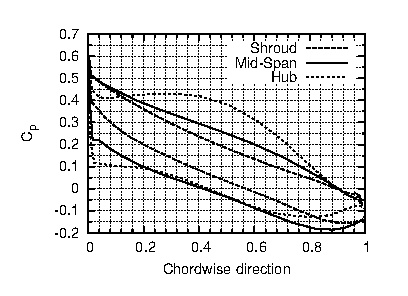
\includegraphics{Load_B3.eps}}
\end{minipage}
\caption{Optimization of a Francis Turbine: $C_p$ profiles hub, mid-span and shroud for archived design B3 at the BE point.}
\label{Francis-B3-LOAD}
\end{figure}

The fact that none of the three archived designs neither shows good outlet velocity profiles and loading qualities and that they do not respect the imposed constraints reveals the necessity of a ``revise'' step. In this thesis, this step is based on EAs with or without metamomdels. So practically, two optimizations have been carried out. The first is utilizing a conventional EA ($\mu=30,\lambda=120$) using $336$ design variables, according to the aforementioned parameterization. The second employed the proposed KBD method, i.e. the so-called MAEA(KBD) ($\mu=20,\lambda=60,\lambda_e= 4 ~ to~ 8$, with the IPE phase starting after recording the first $150$ non-failed individuals in the DB). The MAEA(KBD) run used $19$ optimization variables. For both optimizations, the three archived designs are injected in the first generation population.

Regarding KBD, the $19$ optimization variables result from the grouping of the design variables (eq. \ref{non-linear2}) into $6$ groups (table \ref{design_groups}), plus the extrapolation variable $\Psi$. This arrangement generated $6$ weights controlling the influence of each one of the archived designs to any candidate solution, giving rise to $18$ weights in total. The $18$ weights plus $\Psi$ are the $19$ optimization variables.         


\begin{table}[h!]
\begin{center}
\begin{tabular}{ |c|l| }
\hline

Group              & Design variables determining the:\\
\hline
1 & spanwise distributions of $\theta_{LE}$\\
\hline
1 & spanwise distributions of $\theta_{TE}$\\
\hline
2 & spanwise distributions of $\beta_{LE}$\\
\hline
2 & spanwise distributions of $\beta_{TE}$\\
\hline
3 & spanwise distributions of $\zeta_{LE}$\\
\hline
3 & spanwise distributions of $\zeta_{TE}$\\
\hline
4 & spanwise thickness distributions for PS \\
\hline
4 & spanwise thickness distributions for SS\\
\hline
5 & LE meridional position\\
\hline
5 & TE meridional position\\
\hline
5 & shroud meridional generatrices \\
\hline
5 & hub meridional generatrices\\
\hline
6 & water-foil profiles for the PS (11 profiles)\\
\hline
6 & water-foil profiles  for the SS (11 profiles)\\
\hline
\hline
6 & Groups, in total \\
\hline   
\end{tabular}
\caption{
Optimization of a Francis Turbine: The $6$ Groups  defining the $6 \times 3=18$ optimization variables out of the $19$ used in the KBD method.}
\label{design_groups}
\end{center}
\end{table}

The comparison of the performance of EA and MAEA(KBD) is done using the hypervolume indicator \cite{Zitz2007}. The hypervolume indicator assumes that the quality of a Pareto front can be expressed by a scalar value which stands for the area or volume ore hypervolume of the dominated, by the Pareto front, portion of the objective space up to a user-defined nadir point. With the same nadir point, the higher the hypervolume indicator, greater the quality of the Pareto front is.

The comparison of the evolution of the hypervolume indicator in terms of the number of exact evaluations carried out by the EA and the MAEA(KBD) are shown in figure \ref{Francis-Res}. The horizontal axis express the CPU cosy, by just making the realistic assumption that all evaluations have the same cost. 

\begin{figure}[h!]
\begin{minipage}[b]{1\linewidth}
 \centering
 \resizebox*{12.0cm}{!}{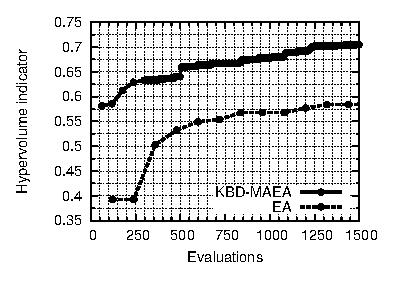
\includegraphics{HypComp.eps}}
\end{minipage}
\caption{Optimization of a Francis Turbine: hypervolume comparison between EA and the proposed MAEA(KBD) method.}
\label{Francis-Res}
\end{figure}

The MAEA(KBD) method significantly outperforms the conventional EA. It starts with significantly better individuals in the first generation which demonstrates that, even though the archived designs are far from the optimal design, the grouping of the design variables and the use of normal distribution to set the importance regions in the design space are very close to the  ``physics'' of the problem in hand.    

\begin{figure}[h!]
\begin{minipage}[b]{1\linewidth}
 \centering
 \resizebox*{13.0cm}{!}{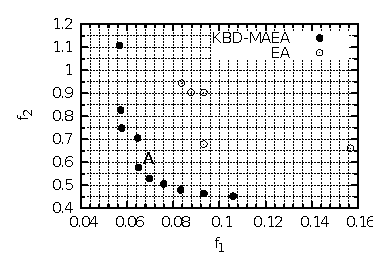
\includegraphics{Comp.eps}}
\end{minipage}
\caption{Optimization of a Francis Turbine: Fronts of non-dominated solutions computed at the cost of $1500$ exact evaluations by the EA and MAEA(KBD) method. The optimal solution A was selected from further analysis (see figures \ref{design-bases-a} to \ref{Francis-A-LOAD}).}
\label{Francis-Res-par}
\end{figure}

By examining fronts of non-dominated solutions (fig. \ref{Francis-Res-par}), as computed by the two methods at the same CPU cost of $1500$ exact evaluations, it can easily be concluded that designs of higher quality were obtained by the MAEA(KBD) method. 
One of the non-dominated solutions computed by the MAEA(KBD), i.e. the one marked with A, was chosen for further analysis at the three operating points.


\begin{figure}[h!]
\begin{minipage}[b]{1\linewidth}
 \centering
 \resizebox*{12.0cm}{!}{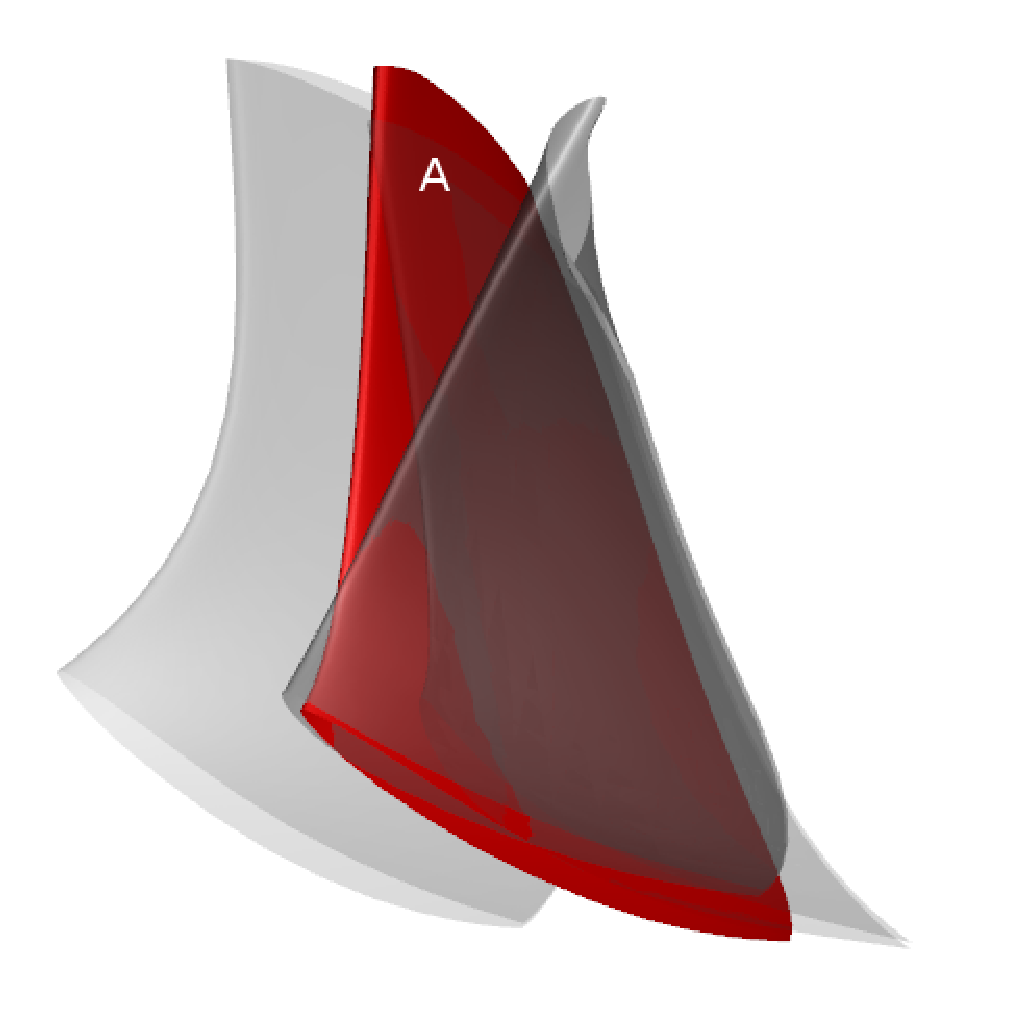
\includegraphics{final.eps}}
\end{minipage}
\caption{Optimization of a Francis Turbine: Design A and the three archived designs used. The high diversity among the four designs can be observed. The ability of the KBD method to produce designs highly diversed in comparison with the archived ones is noticeable.}
\label{design-bases-a}
\end{figure}

The quality metrics of design A are summarized in table \ref{Asum}. To compare design A with the archived ones, its metrics should be compared with the values in table \ref{reuse}. This comparison reveals that, design A is significantly better that the three archived designs at all operating points and for both objectives. Design A is, in fact, a high quality blade.


\begin{table}[h!]
\begin{center}
\begin{tabular}{ |c|c|c|c|c|c| }
\hline
Geometry & OP & $M_1$ & $M_2$  & $\sigma_i^{Hist}$ & $|\delta H|$\\
\hline
& BE & $0.001$ & $0.302$ & $0.18 < 0.2$ & $ 1.1\% <1.5\%$ \\
A & PL & $0.086$ & $0.409$ & $0.19 < 0.2$ & $ 1.5\% <5\%$ \\
& FL & $0.092$ & $0.504$ & $0.18 < 0.2$ & $ 4.1\% <5\%$  \\
\hline
\end{tabular}
\caption{Optimization of a Francis Turbine: Quality metrics (objectives and constraints) regarding the chosen design A for all operating points (BE,PL $\&$ FL). The design is safe from cavitation at all operating points and operates within the desirable range.}
\label{Asum}
\end{center}
\end{table} 

Regarding cavitation, the behaviour of the selected design A can be seen by examining figures \ref{Francis-A-BE}, \ref{Francis-A-PL} and \ref{Francis-A-FL}, for the BE, PL and FL points, respectively.      


\begin{figure}[h!]
\begin{minipage}[b]{1\linewidth}
 \centering
 \resizebox*{14.0cm}{!}{\includegraphics{ABE.eps}}
\end{minipage}
\caption{Optimization of a Francis Turbine: $C_p$ contour for design A at BE operating point. The lowest $C_p$ value is equal to $-0.179$ suggesting a $\sigma_i$ value of $0.179$ well below the $0.2$  imposed cavitation limit.}
\label{Francis-A-BE}
\end{figure}

At the BE point, the lowest $C_p$ value is $-0.179$, see figure \ref{Francis-A-BE}, suggesting the absence of cavitation.
At the PL point, the lowest $C_p$ value is $-0.192$ and, therefore, $\sigma_i \approx 0.192$ which is quite close to the $0.2$ limit but still safe. Typically, off-design points, such as the PL and the FL ones, operate closer to the cavitation limit than the BE one. Design A, when operating at PL, yields the lowest values of $C_p$ at the suction side of the blade near the trailing edge, figure \ref{Francis-A-PL}.  
Regarding the FL point, the lowest  $C_p$ value is equal to $-0.182$ (figure \ref{Francis-A-FL}). Figure \ref{Francis-A-SS} demonstrates that the blade areas which are prone to cavitation are close to the trailing and the leading edges, on the suction side. 

 
\begin{figure}[h!]
\begin{minipage}[b]{1\linewidth}
 \centering
 \resizebox*{14.0cm}{!}{\includegraphics{APL.eps}}
\end{minipage}
\caption{Optimization of a Francis Turbine: $C_p$ contour for design A at PL operating point. The lowest $C_p$ value is equal to $-0.192$ which compared to the BE point operation, figure \ref{Francis-A-BE}, is quite closer to the cavitation threshold but still on the safe side.}
\label{Francis-A-PL}
\end{figure}


\begin{figure}[h!]
\begin{minipage}[b]{1\linewidth}
 \centering
 \resizebox*{14.0cm}{!}{\includegraphics{AFL.eps}}
\end{minipage}
\caption{Optimization of a Francis Turbine: $C_p$ contour for design A at FL operating point over suction side. The lowest  $C_p$ value is $-0.182$, which is lower than the operation at the BE point, but not lower than the PL one.}
\label{Francis-A-FL}
\end{figure}


\begin{figure}[h!]
\begin{minipage}[b]{1\linewidth}
 \centering
 \resizebox*{14.0cm}{!}{\includegraphics{ASS.eps}}
\end{minipage}
\caption{Optimization of a Francis Turbine: $C_p$ contour for design A at the FL operating point. A closer loot at the suction side of the blade when operating at the FL point demonstrates an additional low $C_p$ zone, apart from close to the trailing edge, near the leading edge. }
\label{Francis-A-SS}
\end{figure}

Furthermore, the outlet flow quality of design A at the BE point is plotted in figure  \ref{Francis-A-OUT}. Design A clearly outperforms all three archived designs regarding the outlet quality metric. Since a quite good agreement  with the desirable outlet $C_m$ and $C_u$ distributions is obtained.

\begin{figure}[h!]
\begin{minipage}[b]{1\linewidth}
 \centering
 \resizebox*{11.0cm}{!}{\includegraphics{OUTLET_A.eps}}
\end{minipage}
\caption{Optimization of a Francis Turbine: Exit $C_m$ and $C_u$ profiles for design A, at the BE point.}
\label{Francis-A-OUT}
\end{figure}

For the same design, its loading quality at hub, mid-span and shroud is presented in figure \ref{Francis-A-LOAD}).

\begin{figure}[h!]
\begin{minipage}[b]{1\linewidth}
 \centering
 \resizebox*{11.0cm}{!}{\includegraphics{Load_A.eps}}
\end{minipage}
\caption{Optimization of a Francis Turbine: $C_p$ profiles hub, mid-span and shroud, for design A, at the BE point.}
\label{Francis-A-LOAD}
\end{figure} 

\clearpage

\section{Optimization of a Hydromatrix$\circledR$ Turbine}
\label{Matrix-case}
In this section, the design-optimization of a complete Hydromatrix$\circledR$ turbine will be presented. This case will be used to demonstrate expected gain from the use of the proposed MAEA(PCA) method. Many industrial optimization problems, such as the design of a  Hydromatrix$\circledR$ turbine, are ill-posed which, as shown in chapter 4, cause performance degradation in EAs.   
\subsection{The Hydromatrix$\circledR$ turbine}
Hydromatrix$\circledR$ is an axial reaction type water turbine (fig.\ref{Matrix_c}) developed by Andritz Hydro as an innovative solution for low head hydropower sites \cite{matrix,matrix_2}. The concept of Hydromatrix$\circledR$ relies on the use of a number of small non-regulated (fixed blade) turbines, in place of a conventional large regulated one (fig.\ref{Matrix_a}).  The proposed way to regulate a Hydromatrix$\circledR$ system is via closing/opening a number of turbines so to keep the massflow per open turbine as close as possible to that of its BE operating point. If the flow exceeds the turbines capacity, in order to avoid flood, a number of turbines can be raised or removed from their operating positions, like a gate (fig.~\ref{Matrix_a}).  


\begin{figure}[h!]
%\begin{minipage}[b]{0.5\linewidth}
% \centering
% \resizebox*{7.0cm}{!}{\includegraphics{Matrix1.eps}}
%\end{minipage}
\begin{minipage}[b]{1.0\linewidth}
 \centering
 \resizebox*{11.0cm}{!}{\includegraphics{Matrix2.eps}}
\end{minipage}
\caption{Optimization of a Hydromatrix$\circledR$ Turbine: Matrix turbine and its main hydraulic parts \cite{matrix,matrix_2}. }
\label{Matrix_c}
\end{figure}

The Hydromatrix$\circledR$ ability to use existing weir structures reduces the  additional civil works to minimum and enables power plant operators to install hydroelectric power plants at extremely competitive costs with minimal environmental impact. The number of matrix turbines and their arrangement in rows depends on the existing civil structure and its position relative to the head- and tail-water elevations. The use of a number of small turbine generator units (also known as “modules”) results in simple and robust turbine and generator design. The standardized modular factory assembled grid or “matrix” (fig.~\ref{Matrix_a}) results in short project schedules and high availability. A Hydromatrix$\circledR$ turbine consists of three different parts: the distributor cone containing the stay-wanes, the runner and the draft-tube (fig.\ref{Matrix_c}).



\begin{figure}[h!]
\begin{minipage}[b]{0.5\linewidth}
 \centering
 \resizebox*{7.0cm}{!}{\includegraphics{Matrix3.eps}}
\end{minipage}
\begin{minipage}[b]{0.5\linewidth}
 \centering
 \resizebox*{7.0cm}{!}{\includegraphics{Matrix4.eps}}
\end{minipage}
\caption{Optimization of a Hydromatrix$\circledR$ Turbine: Left; replacement of a single large turbine by a matrix of smaller ones. Right; Matrix turbines in raised position (in case of flood conditions, inspection or maintenance).}
\label{Matrix_a}
\end{figure}

%In order to achieve technical and economical feasible applications, the following main conditions have to be observed \cite{matrix,matrix_2}: 
The technical requirements regarding the economically feasible use of Hydromatrix$\circledR$ are listed below \cite{matrix,matrix_2}: 
\begin{itemize}
\item Available plant discharge greater than $60 m^3/s$. 
\item Available head from 2 to 30 m. 
\item Minimum submergence 1.5 m below tailwater.
\item Unit output from 200 kW up to 700 kW.
\item Close grid connection.
\item Structure available $\&$ suitable for Hydromatrix$\circledR$. 
\begin{itemize}
	\item Navigation dams: large lock $\&$ dams navigational structures along a number of major rivers. 
	\item Irrigation dams: Many structures are existing for irrigation purposes worldwide, spilling water to agricultural areas on a regular basis.
	\item Sluice in shiplocks: Navigation river systems include dams and locks for ship transfer. Where an existing slot is available, a HYDROMATRIX $\circledR$ module can be installed for power generation. The turbine-generator units can be designed to operate in both flow directions. 
	\item Abandoned shiplocks: Due to increasing navigation and transport activities on major rivers, the original shiplocks have become too small and new shiplocks were built.
\end{itemize}
\end{itemize}

\subsection{Case presentation}
This section is concerned with the design of a complete Hydromatrix$\circledR$ turbine for a given hydroelectric plant. The fact that Hydromatrix$\circledR$ is a new type of hydro turbine and that within their operating range lays a high number of untapped locations worldwide denotes the importance of this kind of design-optimization cases for the hydraulic turbine industry.    


\subsubsection{Case formulation}
The design problem in hand consists of the design of the rotor blades, rotor hub and stay-vane end-tips. The distributor cone, the runner shroud and the draft tube are fixed due to the modular construction and the generator size (fig.\ref{Matrix_b}).     


\begin{figure}[h!]
\centering
\includegraphics[width=120mm]{gen_turb.eps}    
\caption{Optimization of a Hydromatrix$\circledR$ Turbine: Matrix turbine schematic representation, with red are the free to design parts and black are the fixed due to construction constraints parts.  }
\label{Matrix_b}
\end{figure}

\subsubsection{Design parameterization}
In this case, the vector of design variables could be decomposed into two parts, one which is associated with the runner blade and the hub and another one associated with the stay-vanes. The first part is based on the parameterization presented in section \ref{Paramt} and introduces $52$ design variables to describe the rotor blade mean surface, its thickness distribution and, also, define the hub generatrices (table. \ref{design_vars2}). The second part of the parameterization is associated solely with the stay-vane TE, since the stay-vanes thickness distributions are frozen for reasons related to their structural behaviour (stay-vanes must hold both the generator and runner weight in place). Also, the stay-vane LE is fixed since the flow meets the stay-vanes with a given, axial, velocity.  The EA is concerned only with the first part of the parameterization. The second part is used to regulate the BE operating point as will be shown later.      

\begin{table}[h!]
\begin{center}
\begin{tabular}{ |c|l| }
\hline

Number of              & Design variables determining the:\\
design variables       & \\
\hline
6 & spanwise distributions of $\theta_{LE}$\\
\hline
6 & spanwise distributions of $\theta_{TE}$\\
\hline
6 & spanwise distributions of $\beta_{LE}$\\
\hline
6 & spanwise distributions of $\beta_{TE}$\\
\hline
6 & spanwise distributions of $\zeta_{LE}$\\
\hline
6 & spanwise distributions of $\zeta_{TE}$\\
\hline
%0 & spanwise thickness distributions for PS \\
%\hline
%0 & spanwise thickness distributions for SS\\
%\hline
8 & LE projection on the meridional plane\\
\hline
8 & TE projection on the meridional plane\\
\hline
%0 & shroud generatric(on the meridional plane)  \\
%\hline
%0 & hub generatric(on the meridional plane)\\
%\hline
%$0 \times 11$ & chordwise thikness destribution for PS (11 profiles)\\
%\hline
%$0 \times 11$ & chordwise thikness destribution for SS (11 profiles)\\
%\hline
\hline
$52$ & Design variables, in total \\
\hline   
\end{tabular}
\caption{
The $52$ design variables used to parameterize the Hydromatrix$\circledR$ runner. This is the array of design variables the EA is dealing with.}
\label{design_vars2}
\end{center}
\end{table}

The first step for evaluating the performance of each runner geometry is the numerical simulation of the water flow through the turbine, section \ref{FlowSolvert}. Herein the Euler solver presented in section \ref{FlowSolvert} is used.  The solver uses as input the rotational velocity (n) and the total pressure drop from inlet to outlet (H). For a candidate geometry, the flow rate Q is an outcome of the simulation. To get the desired Q value in order to operate at the BE operating point, a procedure which iteratively deflects the stay-vane TE (second part of the parameterization) is used. This procedure is explained in detail in section \ref{single.regulated}. So, even if the optimization problem deals only with the design of the runner, the trailing part of the stay-vane iteratively adapts it self so to fit the given rotor. The designer defines the maximum number of iterations of the deflection angle $\alpha$ which are allowed to perform before reaching the desired Q value. This iterative process is the main reason that the CPU cost per evaluation may noticeably vary among the candidate solutions.



%\begin{figure}[h!]
%\centering
%\includegraphics[width=100mm]{stator.eps}    
%\caption{Optimization of a Hydromatrix$\circledR$ Turbine: 
%The stator deflection angle $a$ is iteratively adapted to match %%the desired flow rate $Q$. Since this a propeller--type turbine, the iterative correction of $a$ needs to be performed at the peak operating point only. A solution that fails to satisfy the desirable $Q$ value at the peak operating point is not evaluated at the remaining two operating points and is given ``death penalty''.}
%\label{Matrix_stator}
%\end{figure}

\subsubsection{Objectives and Constraints}

The objectives vector consists of two objectives. $f_1$ is the outlet velocity profile metric ($M_1$) and $f_2$ is the combination of (a) blade loading quality metric ($M_2$), (b) the cavitation index $\sigma_i^{Hist}$ and (c) the pumping surface metric ($M_3$). The first objective is, therefore, concerned with the draft-tube coupling quality seeking for blades with the least divergence from the user defined target profiles as they are shown in figure \ref{design-obj-tar-Matrix}. On the other hand, the second objective controls the pressure distribution over the runner blade, incorporating all relevant quality metrics.

\begin{eqnarray}
f_1^i= \alpha ^i M_1^i
%   f_1^i= \alpha ^i  M_1^i ~~~\& ~~~ f_2^i=\beta ^i Μ_2^i-\gamma ^i  \sigma^i + \delta ^i  Μ_3^i 
   \label{ObjM} 
\end{eqnarray}
\begin{eqnarray}
\nonumber
f_2^i =\beta ^i M_2^i +\gamma ^i \sigma_i^{Hist} +\delta ^i M3^i
%   f_1^i= \alpha ^i  M_1^i ~~~\& ~~~ f_2^i=\beta ^i Μ_2^i-\gamma ^i  \sigma^i + \delta ^i  Μ_3^i 
   \label{ObjM} 
\end{eqnarray}


\begin{table}[h!]
\begin{center}
\begin{tabular}{ |l|r|r|r|c| }
%\hline
%\multicolumn{4}{|c|}{Βάρη} & F \\
\hline
& BE, $i\!=\!1$ & PL, $i\!=\!2$ & FL, $i\!=\!3$ &  Contributing to\\
\hline
\greek{α$^i$ ($M_1$)} & 1.0            &0.0            &0.0 & $f_1$\\
\hline
\greek{β$^i$ ($M_2$)} &0.2    &0.0            &0.0  & $f_2$\\
\hline
\greek{γ$^i$ $(\sigma_i^{Hist})$} &1.0            &1.0            &1.0 & $f_2$\\
\hline
\greek{δ$^i$} ($M_3$) &0.0            &100.0  &100.0 & $f_2$\\
\hline
\end{tabular}
\caption{Optimization of a Hydromatrix$\circledR$ Turbine: Weights associated with the quality-metrics for grouping them into the two objective functions $f_1$ and $f_2$.}
\label{op-weights-M1}
\end{center}
\end{table}

\begin{figure}[h!]
\begin{minipage}[b]{1\linewidth}
 \centering
 \resizebox*{10.0cm}{!}{\includegraphics{TargetMatrix.eps}}
\end{minipage}
\caption{Optimization of a Hydromatrix$\circledR$ Turbine: Target nondimensional velocity profile distributions.}
\label{design-obj-tar-Matrix}
\end{figure}

\newpage

For the already defined $3\!\times\!2\!=\!6$ functions to be minimized at the three operating points, the two objective functions used in the optimization problem are defined by concatenating the previous ones with weight factors $w_i$ (table \ref{weights}), as follows

\begin{equation} 
f_1=\sum^3_{i=1}w_if_1^i ~~~\&~~~ f_2=\sum^3_{i=1}w_if_2^i
\label{F12}
\end{equation}


\begin{table}[h!]
\begin{center}
\begin{tabular}{ |c|c| }
\hline
Operating point & weight, $w_i$\\
\hline
Best efficiency (BE), $i\!=\!1$  & 1.0\\
\hline
Part load  (PL), $i\!=\!2$ & 0.1\\
\hline
Full load (FL), $i\!=\!3$  & 0.1\\
\hline
\end{tabular}
\caption{Optimization of a Hydromatrix$\circledR$ Turbine: Operating point weights.}
\label{weights}
\end{center}
\end{table}


\subsection{Results}
As mentioned in the beginning of this section, this case is used to demonstrate the merits of the proposed use of PCA to drive the evolution operators namely the so-called MAEA(PCA) method. Therefore, two optimization runs were performed using the conventional MAEA and the proposed MAEA(PCA).

In both runs the  population sizes were $\mu\!=\!30$ and $\lambda\!=\!90$. In such a problem, the quite high value of the offspring population $\lambda$ is really necessary since the blade shape parameterization and the bounds of the design variables may generate many infeasible solutions  with in the starting population. In more detail, for both runs, $88$ of the $90$ individuals in the first generation correspond to infeasible geometries and they all receive death penalty. If all members of the initial generation receive death penalty then all of them have the same scalar cost function $\Phi$, this can lead to premature evolution stagnation, constantly generating infeasible solutions. The inexact pre-evaluation was adjusted to start once $300$ non-failed individuals entered the DB. Up to $\lambda_e\!=\!18$ top individuals per generation were allowed to undergo re-evaluation on the CFD tool. Locally valid RBF networks were used as metamodels; each metamondel is trained on a few previously evaluated individuals in its vicinity. Based on the algorithm presented in \cite{LTT_2_029}, the designer defines the minimum ($12$) and maximum ($16$) number of training patterns to be used. It is important to note that, due to the very strict constraints, the DB records a great number of previously evaluated solutions which were given ``death penalty''. The presence of so many infeasible entries in the DB can lead to a great number or infeasible entries included in the metamodels training set. This should be avoided since it prevents dependable metamodels to be trained.

The application of the PCA-assisted evolution operators started at the $5^{th}$ generation. In fig.~\ref{hyp_matrix}, the performance of MAEA and MAEA(PCA) are compared, based on the evolution of the hypervolume indicator.


\begin{figure}[h!]
\begin{minipage}[b]{1\linewidth}
 \centering
 \resizebox*{12.0cm}{!}{\includegraphics{nhyperv.eps}}
\end{minipage}
\caption{Optimization of a Hydromatrix$\circledR$ Turbine: The evolution of the hypervolume indicator for (a) the MAEA and (b) the MAEA(PCA) implementing the PCA-assisted evolutionary operators. It is evident that, since the PCA--assisted operators apply at the ($5^{th}$) generation, i.e. after about $4\!\times\!90\!=\!360$ evaluations based on the CFD tool, the first parts of the two curves are identical.}
\label{hyp_matrix}
\end{figure}
 
MAEA(PCA) constantly finds a better front of non-dominated solutions during the entire course of evolution, at the same computational cost. From a different point of view, the quality of the front of non-dominated solutions obtained by MAEA after $2000$ CFD-based evaluations can be  obtained at less than half this CPU cost by the MAEA(PCA). 

\begin{figure}[h!]
\begin{minipage}[b]{1\linewidth}
 \centering
 \resizebox*{12.0cm}{!}{\includegraphics{fparetos.eps}}
\end{minipage}
\caption{Optimization of a Hydromatrix$\circledR$ Turbine: Comparison of the fronts of non-dominated solutions computed using MAEA and MAEA(PCA), at the cost of $2000$ CFD--based evaluations.  Abscissa and ordinate correspond to the two objectives, as defined by eqs.~\ref{F12}.}
\label{pareto_matrix}
\end{figure}
 
 
The analysis of the non--dominated solution marked with $A$, fig. \ref{pareto_matrix}, follows. Fig.~\ref{All_press} shows the computed $C_p$ isoareas at BE point, over the entire turbine unit with its stator, rotor, hub and shroud. 

\begin{figure}[h!]
\begin{minipage}[b]{1\linewidth}
 \centering
 \resizebox*{15.0cm}{!}{\includegraphics{AllPress.eps}}
\end{minipage}
\caption{Optimization of a Hydromatrix$\circledR$ Turbine: $C_p$ isoareas for design A, at the BE point.}
\label{All_press}
\end{figure}


The outlet flow quality of design A is presented in fig. \ref{out_MAT}. Target distributions are achieved as desired.
Furthermore the $C_p$ profiles at the hub, mid-span and shroud locations of the blade, at the BE, PL and FL operating points are presented in figures \ref{LOADBEM}, \ref{LOADPLM} and \ref{LOADFLM}, respectively. The inevitable, due to the propeller type of the turbine, pumping surface makes its appearance at the PL point as expected. It is though kept at the minimum possible level. The pumping surface spans from the mid-span to the shroud as can be seen in figure \ref{LOADPLM}. In fact, a small pumping surface is allowed at the PL point given that this is a non-regulated machine.            
%The pumping surface appears close to the shroud region, this is due to the fact that this is the region with the greatest radius thus the region that gets more affected my the change of operating point. In simpler worlds changing the operating point changes, in the grated degree, the angle which the flow meets the runner blade at the near shroud position. This is true for both the FL and PL positions. In order to keep the pick observed at the leading edge near the shroud for the FL operating point a small amount of pumping surface is allowed at the PL operating given that this is a non-regulated machine thus regulation through the stator-wanes is not available.           



\begin{figure}[h!]
\begin{minipage}[b]{1\linewidth}
 \centering
 \resizebox*{11.0cm}{!}{\includegraphics{OUTLETMATRIX.eps}}
\end{minipage}
\caption{Optimization of a Hydromatrix$\circledR$ Turbine: $C_m$ and $C_u$ exit velocity profiles for design A, at the BE point.}
\label{out_MAT}
\end{figure}



\begin{figure}[h!]
\begin{minipage}[b]{1\linewidth}
 \centering
 \resizebox*{11.0cm}{!}{\includegraphics{LoadPL_M.eps}}
\end{minipage}
\caption{Optimization of a Hydromatrix$\circledR$ Turbine: $C_p$ profiles for hub, mid-span and shroud waterfoils of design A operating at the PL point. The pressure overshooting near the LE, at the suction side, due to the negative incidence angle (figure \ref{design-PL-M}), is the reason of the so-called pumping surface phenomenon.}
\label{LOADPLM}
\end{figure}

\begin{figure}[h!]
\begin{minipage}[b]{1\linewidth}
 \centering
 \resizebox*{11.0cm}{!}{\includegraphics{LoadBE_M.eps}}
\end{minipage}
\caption{Optimization of a Hydromatrix$\circledR$ Turbine: $C_p$ profiles for hub, mid-span and shroud positions waterfoils of design A operating at the BE point.}
\label{LOADBEM}
\end{figure}

\begin{figure}[h!]
\begin{minipage}[b]{1\linewidth}
 \centering
 \resizebox*{11.0cm}{!}{\includegraphics{LoadFL_M.eps}}
\end{minipage}
\caption{Optimization of a Hydromatrix$\circledR$ Turbine: $C_p$ profiles for hub, mid-span and shroud waterfoils of design A operating at the FL operating point. Compare to its operation at the BE point, there is a pronounced undershooting close to the LE which can be explained by observing the flow incidence in figure \ref{design-FL-M}).}
\label{LOADFLM}
\end{figure}

The pumping surface phenomenon and it cause is observable in figure \ref{design-PL-M}. Pumping surface is the surface shown in dark blue color on the blades pressure side. This is caused by the negative incidence angle, which means that the flow meets the blade at the suction side just after the LE. This can be observed by comparing figures \ref{design-PL-M}, \ref{design-FL-M}, and \ref{design-BE-M}, for the  PL, FL and BE operating points, respectively. The ``best'' incidence angle is associated with the BE operating point. The FL operating point shows a higher than the BE incidence angle, thus creating a lower pressure region near the LE at the suction side, as can be seen by comparing figures \ref{LOADFLM} and \ref{LOADBEM}. As mentioned above, the PL operating point suffers from negative incidence angle, thus creating a region of higher pressure region near the LE at the suction side (compare figures \ref{LOADPLM} and \ref{LOADBEM}), the so-called pumping surface phenomenon.    



\begin{figure}[h!]
\begin{minipage}[b]{1\linewidth}
 \centering
 \resizebox*{15.0cm}{!}{\includegraphics{PartLoad.eps}}
\end{minipage}
\caption{Optimization of a Hydromatrix$\circledR$ Turbine: Computed isobar areas for design A operating at the PL point. The streamlines of the water flow, near the shroud region, reveal the negative local incidence angle (flow meets the blade at the suction side), which causes the pumping surface phenomenon. }
\label{design-PL-M}
\end{figure}


\begin{figure}[h!]
\begin{minipage}[b]{1\linewidth}
 \centering
 \resizebox*{15.0cm}{!}{\includegraphics{BE.eps}}
\end{minipage}
\caption{Optimization of a Hydromatrix$\circledR$ Turbine: Computed isobar areas for design A operating at the BE point. Water streamlines near the shroud region lead to ``better'' flow incidence angle in comparison with the PL operation.}
\label{design-BE-M}
\end{figure}


\begin{figure}[h!]
\begin{minipage}[b]{1\linewidth}
 \centering
 \resizebox*{15.0cm}{!}{\includegraphics{FL.eps}}
\end{minipage}
\caption{Optimization of a Hydromatrix$\circledR$ Turbine: Computed isobar areas for design A operating at the FL point. Water streamlines of the  reveal a higher than the BE incidence angle, which causes a low pressure region near the LE at the suction side, figure \ref{LOADFLM}. }
\label{design-FL-M}
\end{figure}


% ---------------------------------------------------------------------------
% ----------------------- end of thesis sub-document ------------------------
